\subsection{Description}

The dataset is composed of 46 different solutions at different radii.
Each of them is then composed of lists of several observables of different lengths (varying from 15 to 20 entries each, as shown in \Cref{fig:lumps:length}).

\begin{figure}[htbp]
  \centering
  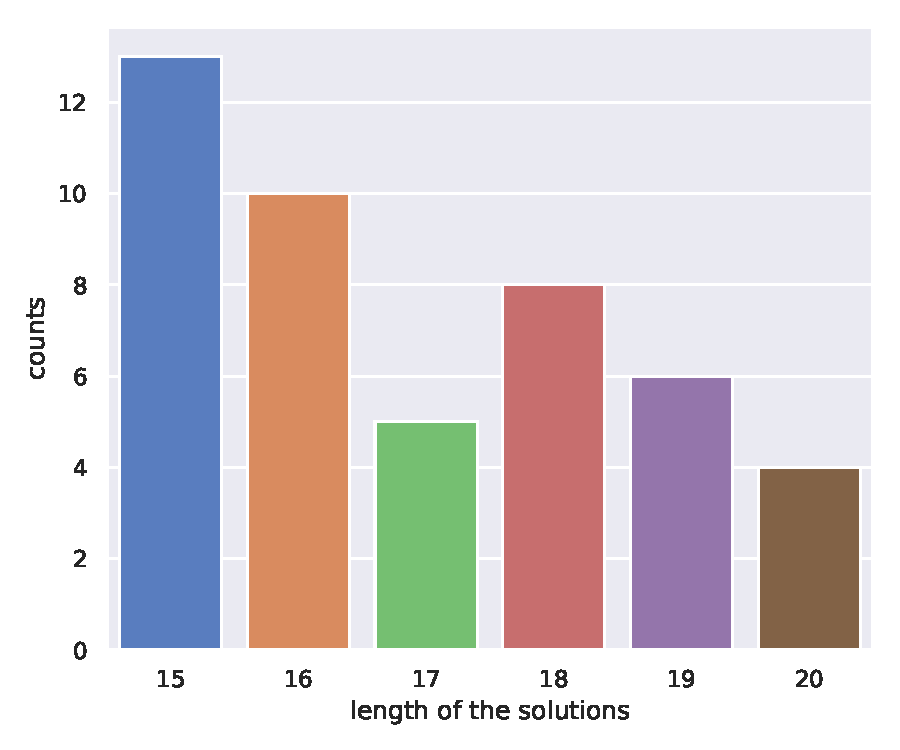
\includegraphics[width=0.6\textwidth]{img/sol_length}
  \caption{Length of the vector-like solutions in the untidied dataset.}
  \label{fig:lumps:length}
\end{figure}

Every observable is characterised by its conformal weight (the \texttt{weight} column in the dataset), its kind of ``oscillations'' (the \texttt{type} variable, categorical and in lexicographic order), its initialisation point (\texttt{init}) and the truncation levels (from level 2 to level 18).
The \texttt{exp} column contains the label to be predicted from the other variables at finite mass level truncation.
It represents the extrapolation at $\infty$ mass level truncation and takes integer values in the range $[-1, 1]$.
In general the entries are real numbers.


\subsection{Preparation}

The entries of the dataset are vector-like objects which need to be tidied before using them for the analysis.
We first artificially insert a new variable (called \texttt{solutions}) to label the 46 different rows of the dataset.
We then flatten the entire dataset over the values in its rows and create a new table containing only numeric entries: the newly formed dataset has 778 rows and 22 columns.

Before proceeding to the analysis we take into account the possibility of relations between the entries and remove the duplicates from the dataset.
In total we remove 46 duplicates corresponding to \SI{6}{\percent} circa of the total dataset.
After this operation the dataset contains 732 rows and it is ready for the \eda.


\subsection{Exploratory Data Analysis}

In the \eda section we study the properties of the tidy dataset.
We focus on outlier detection and correlations between the variables.
We also anticipate that in general we will not use the variables \texttt{init} and \texttt{solutions} since results should not depend on the particular solution or initial value.


\subsubsection{Outliers Detection}

The dataset presents several variables having a very large range of variability and may thus contain a large number of outliers.
As a first step we define the \emph{interquartile} range for each variable and compute the fraction of outlying samples.\footnotemark{}
In general the truncation levels show a high number of outliers (the last truncation level contains \SI{27}{\percent} outlying values, while others have fractions of \SI{20}{\percent} outliers in average).
\footnotetext{%
  To compute the interquartile range we first compute the 25th and 75th percentiles (i.e.\ the first and third quartiles) of the distribution of each variable.
  The range is then defined as \num{1.5} times the distance between the two quartiles computed from the lower and the upper bounds of the distribution of the values.
}

\begin{figure}[htbp]
  \centering
  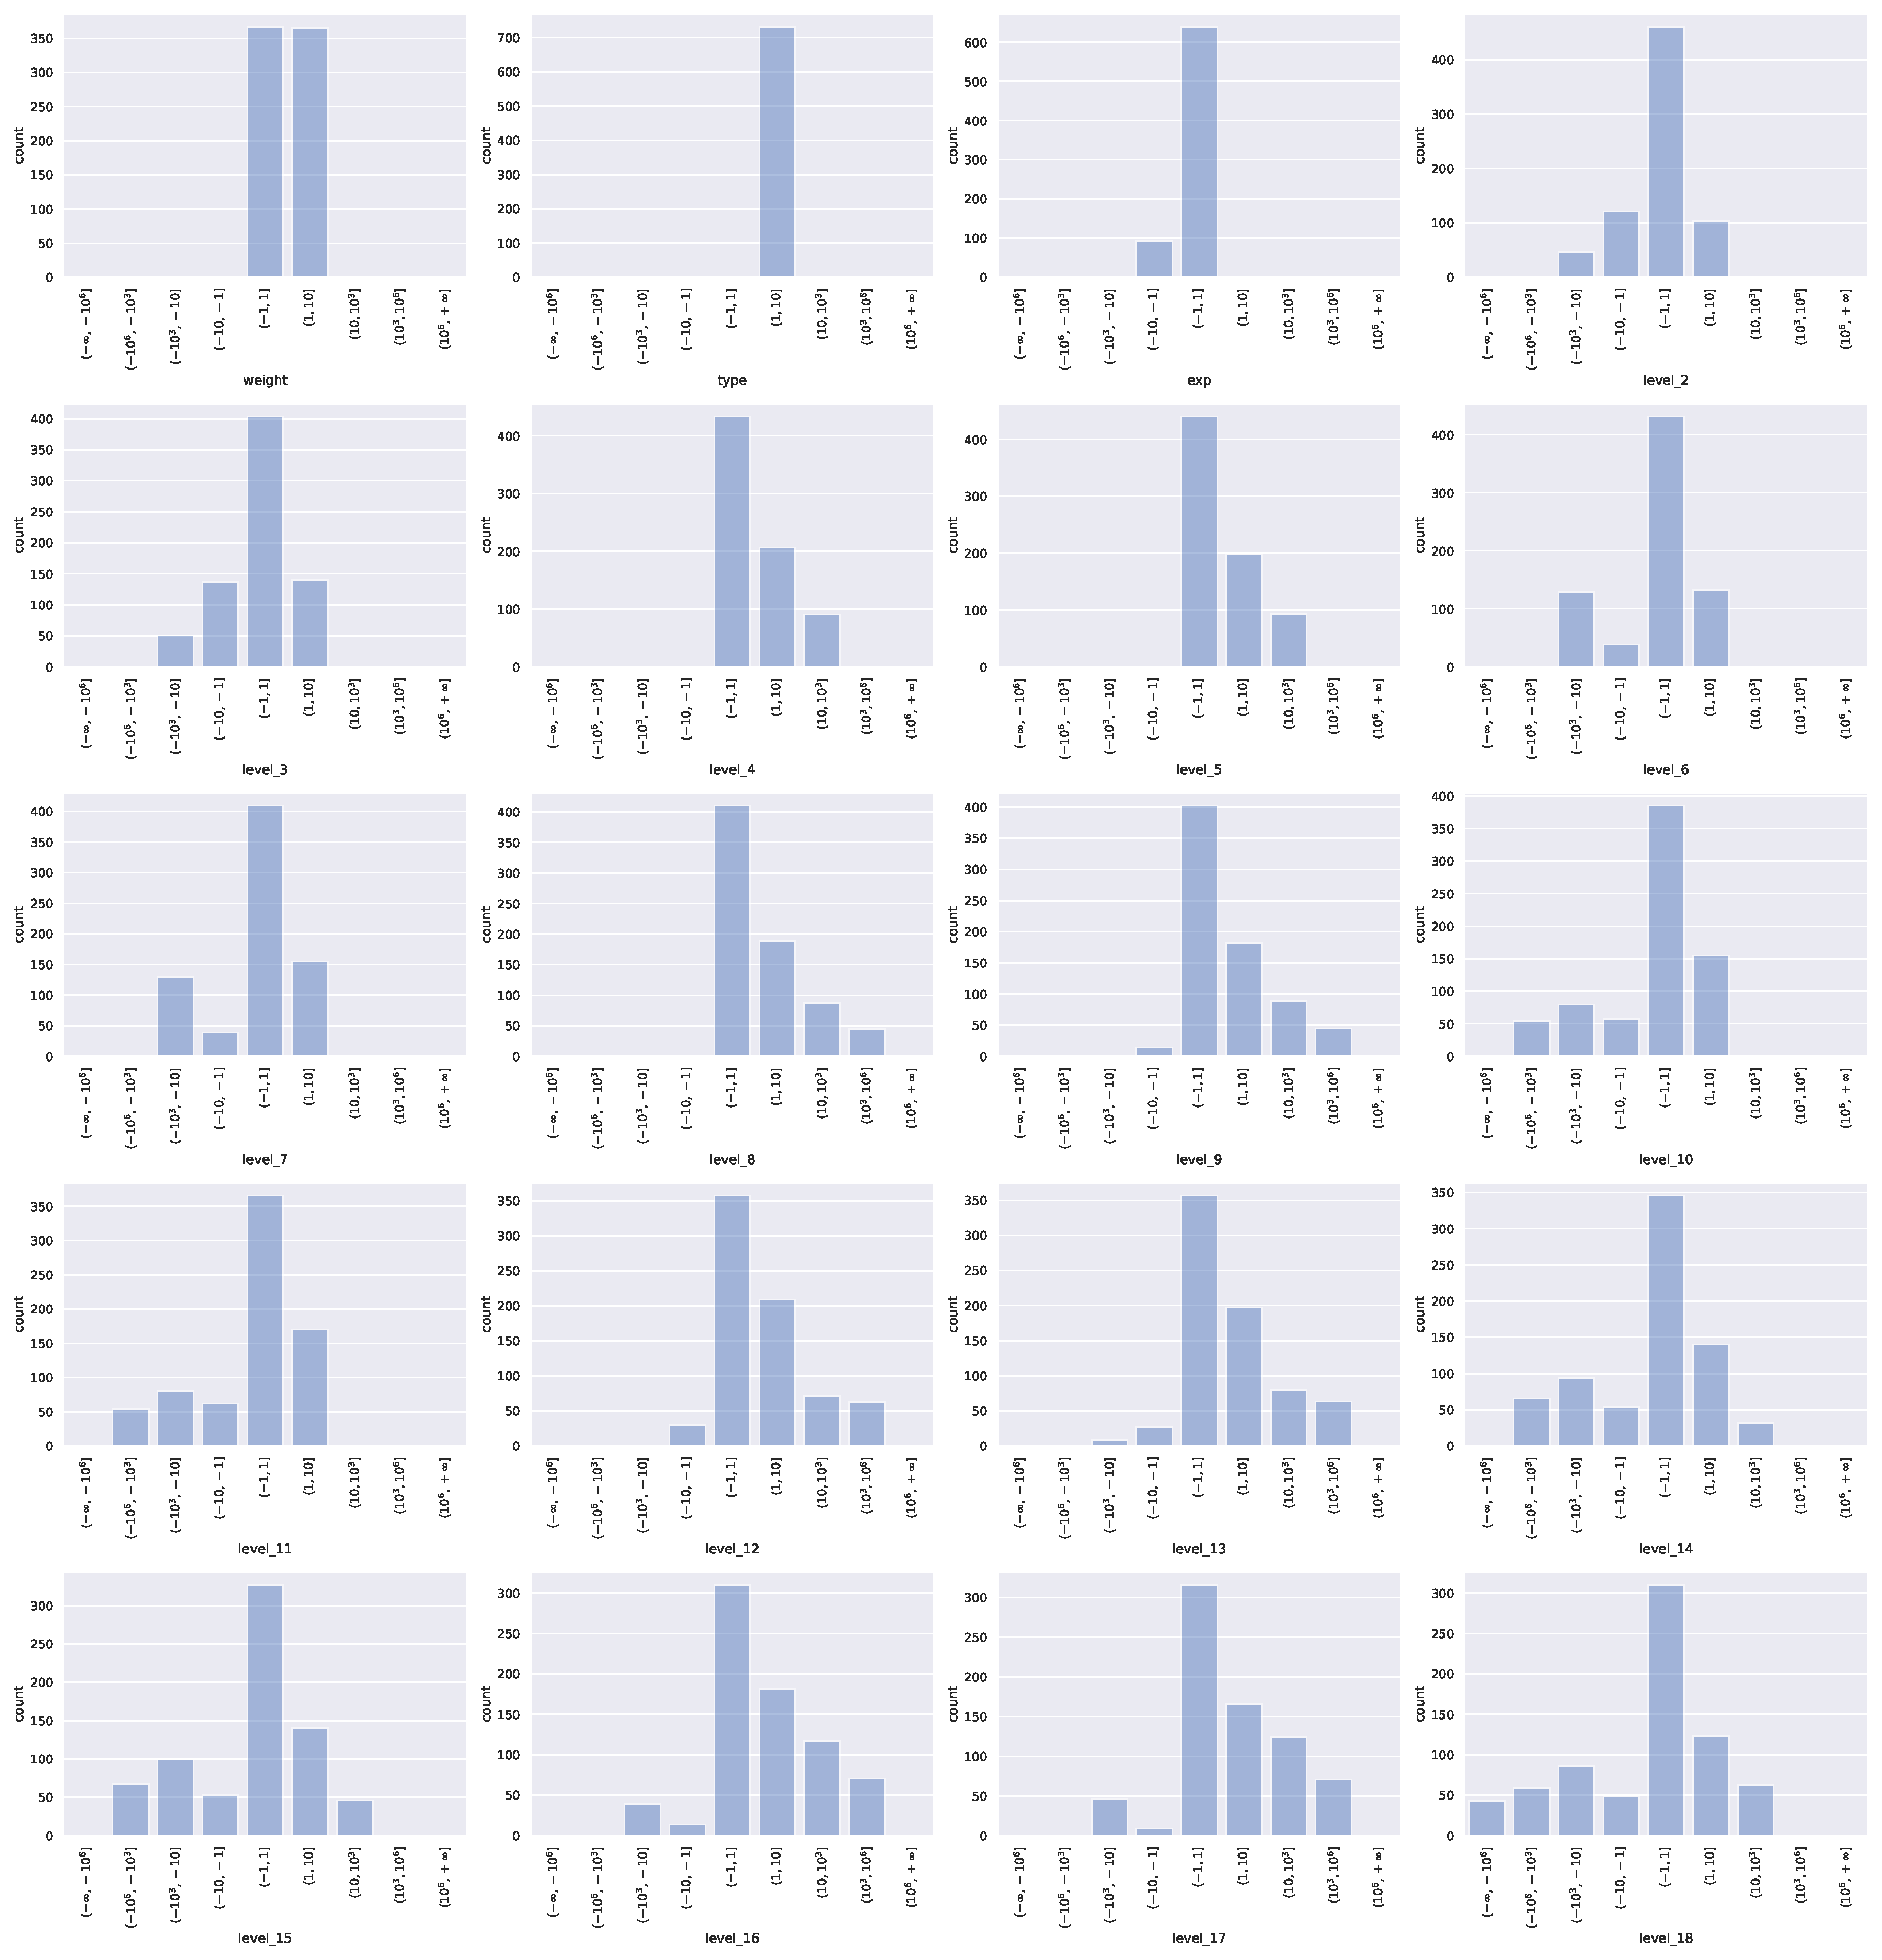
\includegraphics[width=0.6\textwidth]{img/counts_full}
  \caption{Distribution of the values of each variable categorised by order of magnitude.}
  \label{fig:lumps:counts}
\end{figure}

In \Cref{fig:lumps:counts} we show the distribution of the values: in general they are spread across different orders of magnitude and show a tendency to alternate between positive and negative values.
This in turn may cause issues when training \ml algorithms since the very large variance may result in ``too precise'' determination of the coefficients, ultimately leading to a poor generalisation ability.

However the large number of outliers is mainly due to data corresponding to higher values of \texttt{weight}.
In fact we can separately analyse the dataset for \texttt{weight} $< 1.5$ and \texttt{weight} $\ge 1.5$.
In the first case the values of the variables are in general contained in smaller intervals and present a smaller value of the variance as pictorially shown in \Cref{fig:lumps:box}, where we can see that the variables are in general $\order{1}$ in values.
In the latter the distribution is less uniform and encompasses multiple orders of magnitude (differently from the \texttt{weight} $< 1.5$ case showing a box plot similar to \Cref{fig:lumps:box} does not help in visualising the situation).

\begin{figure}[htbp]
  \centering
  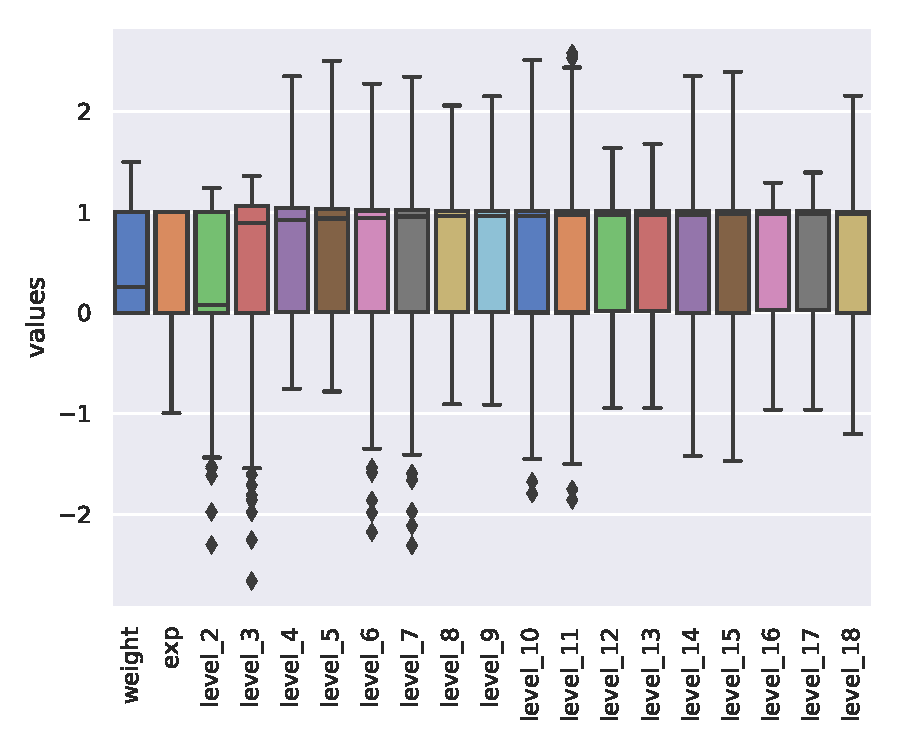
\includegraphics[width=0.6\textwidth]{img/boxplot_low}
  \caption{%
    Boxplot of the values for \texttt{weight} $< 1.5$.
    The coloured boxes represent data between the first and third quartiles (the horizontal line is the median), while the ``whiskers'' show the interquartile range.
    Isolated points are the outliers.
  }
  \label{fig:lumps:box}
\end{figure}

This might be connected to particular relations between the observables. The \eda can highlight some of them (see \Cref{tab:lumps:rel}).
In fact higher weights present only a specific type of oscillation (\texttt{type} is strictly 4), while lower values of \texttt{weight} show that the variables include different kind of oscillations.
However in this case \texttt{type} $= 2$ strictly implies a vanishing weight.

\begin{table}[htbp]
  \centering
  %\resizebox{\textwidth}{!}{%
  \begin{tabular}{@{}cccc@{}}
                     \toprule
                     &               & \multicolumn{2}{c}{\textbf{weight}} \\
  \textbf{weight}    & \textbf{type} & $\mu$             & $\sigma$        \\ \midrule
  \multirow{2}{*}
  {$\ge 1.5$}        & 2             & ---               & ---             \\
                     & 4             & 4                 & 2               \\
  \multirow{2}{*}
  {$< 1.5$}          & 2             & 0                 & 0               \\
                     & 4             & 0.6               & 0.5             \\ \bottomrule
  \end{tabular}%
  %}
  \caption{%
    Relations between the \texttt{type} and \texttt{weight} variables ($\mu$ is its average value and $\sigma$ its standard deviation).
  }
  \label{tab:lumps:rel}
\end{table}

Finally in \Cref{fig:lumps:corr} we show the correlation matrices of the variables.
As expected, the truncation levels are strongly correlated among themselves and with the \texttt{weight} variable.
Though milder, there is also a good correlation of the variables with the labels we intend to predict (\texttt{exp}), while the \texttt{type} variable seems to be completely uncorrelated (this may however be due to the fact of being categorical: a linear regression might be more suitable to do statistical inference on it).
Another notable remark is the different behaviour of the correlations between consecutive layers: the large anti-correlations seem to be entirely due to the higher weights, while \texttt{weight} $< 1.5$ seems to imply a correlation only between adjacent couples of levels (e.g.\ 2-3, 4-5, 6-7, etc.) and their replicas at distance 3 (e.g.\ 4-5 with 8-9, 12-13 and 16-17, 6-7 with 10-11, 14-15 and 18, etc.).
This behaviour may point to several possible interpretations.
In particular we see that data is oscillating: going towards larger truncation levels data seem to alternate a behaviour similar to a periodic function (sine or cosine in the particular case) with maxima and minima alternating at constant intervals.
This may become clear when considering the definition of the correlation factor of two variables $X_1$ and $X_2$ given as the ratio between the covariance $\sigma(X_1,X_2) = (X_1 - \bar{X}_1) \cdot (X_2 - \bar{X}_2)$, where $\bar{X}_1$ and $\bar{X}_2$ are the mean of the respective variables, and the product of the separate standard deviations $\sigma(X_1) \sigma(X_2)$).
However we also see that this behaviour is particularly present when considering the full dataset (or just \texttt{weight} $\ge 1.5$) while if we introduce a cut at \texttt{weight} $< 1.5$ the correlation is definitely less marked, though present.

\begin{figure}[htbp]
  \centering
  \begin{subfigure}{0.32\textwidth}
    \centering
    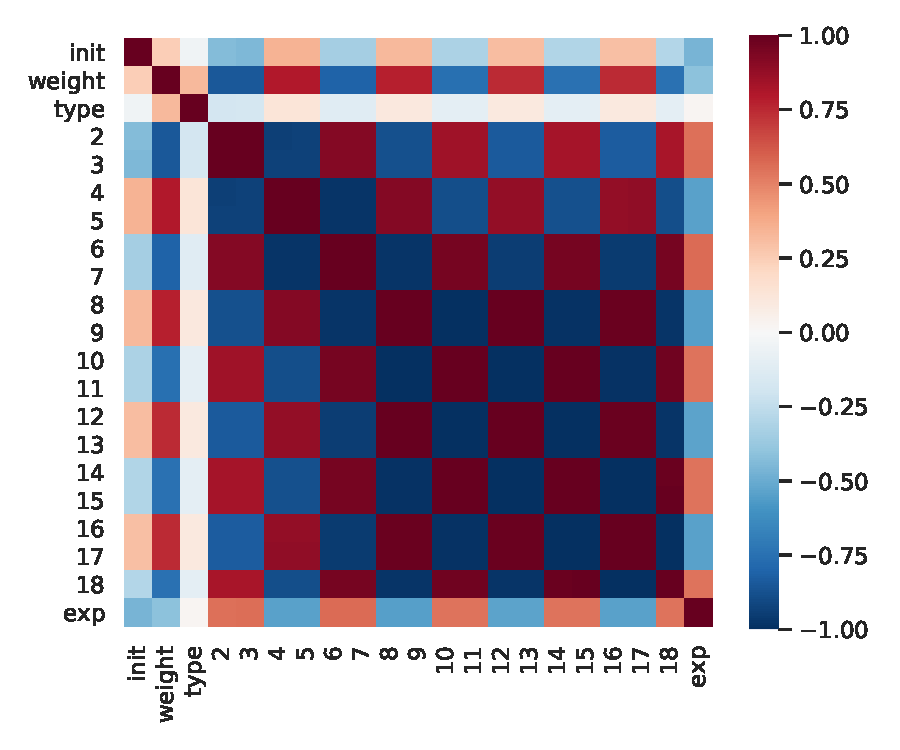
\includegraphics[width=\linewidth]{img/corr_mat_full}
    \caption{Full dataset}
  \end{subfigure}
  \begin{subfigure}{0.32\textwidth}
    \centering
    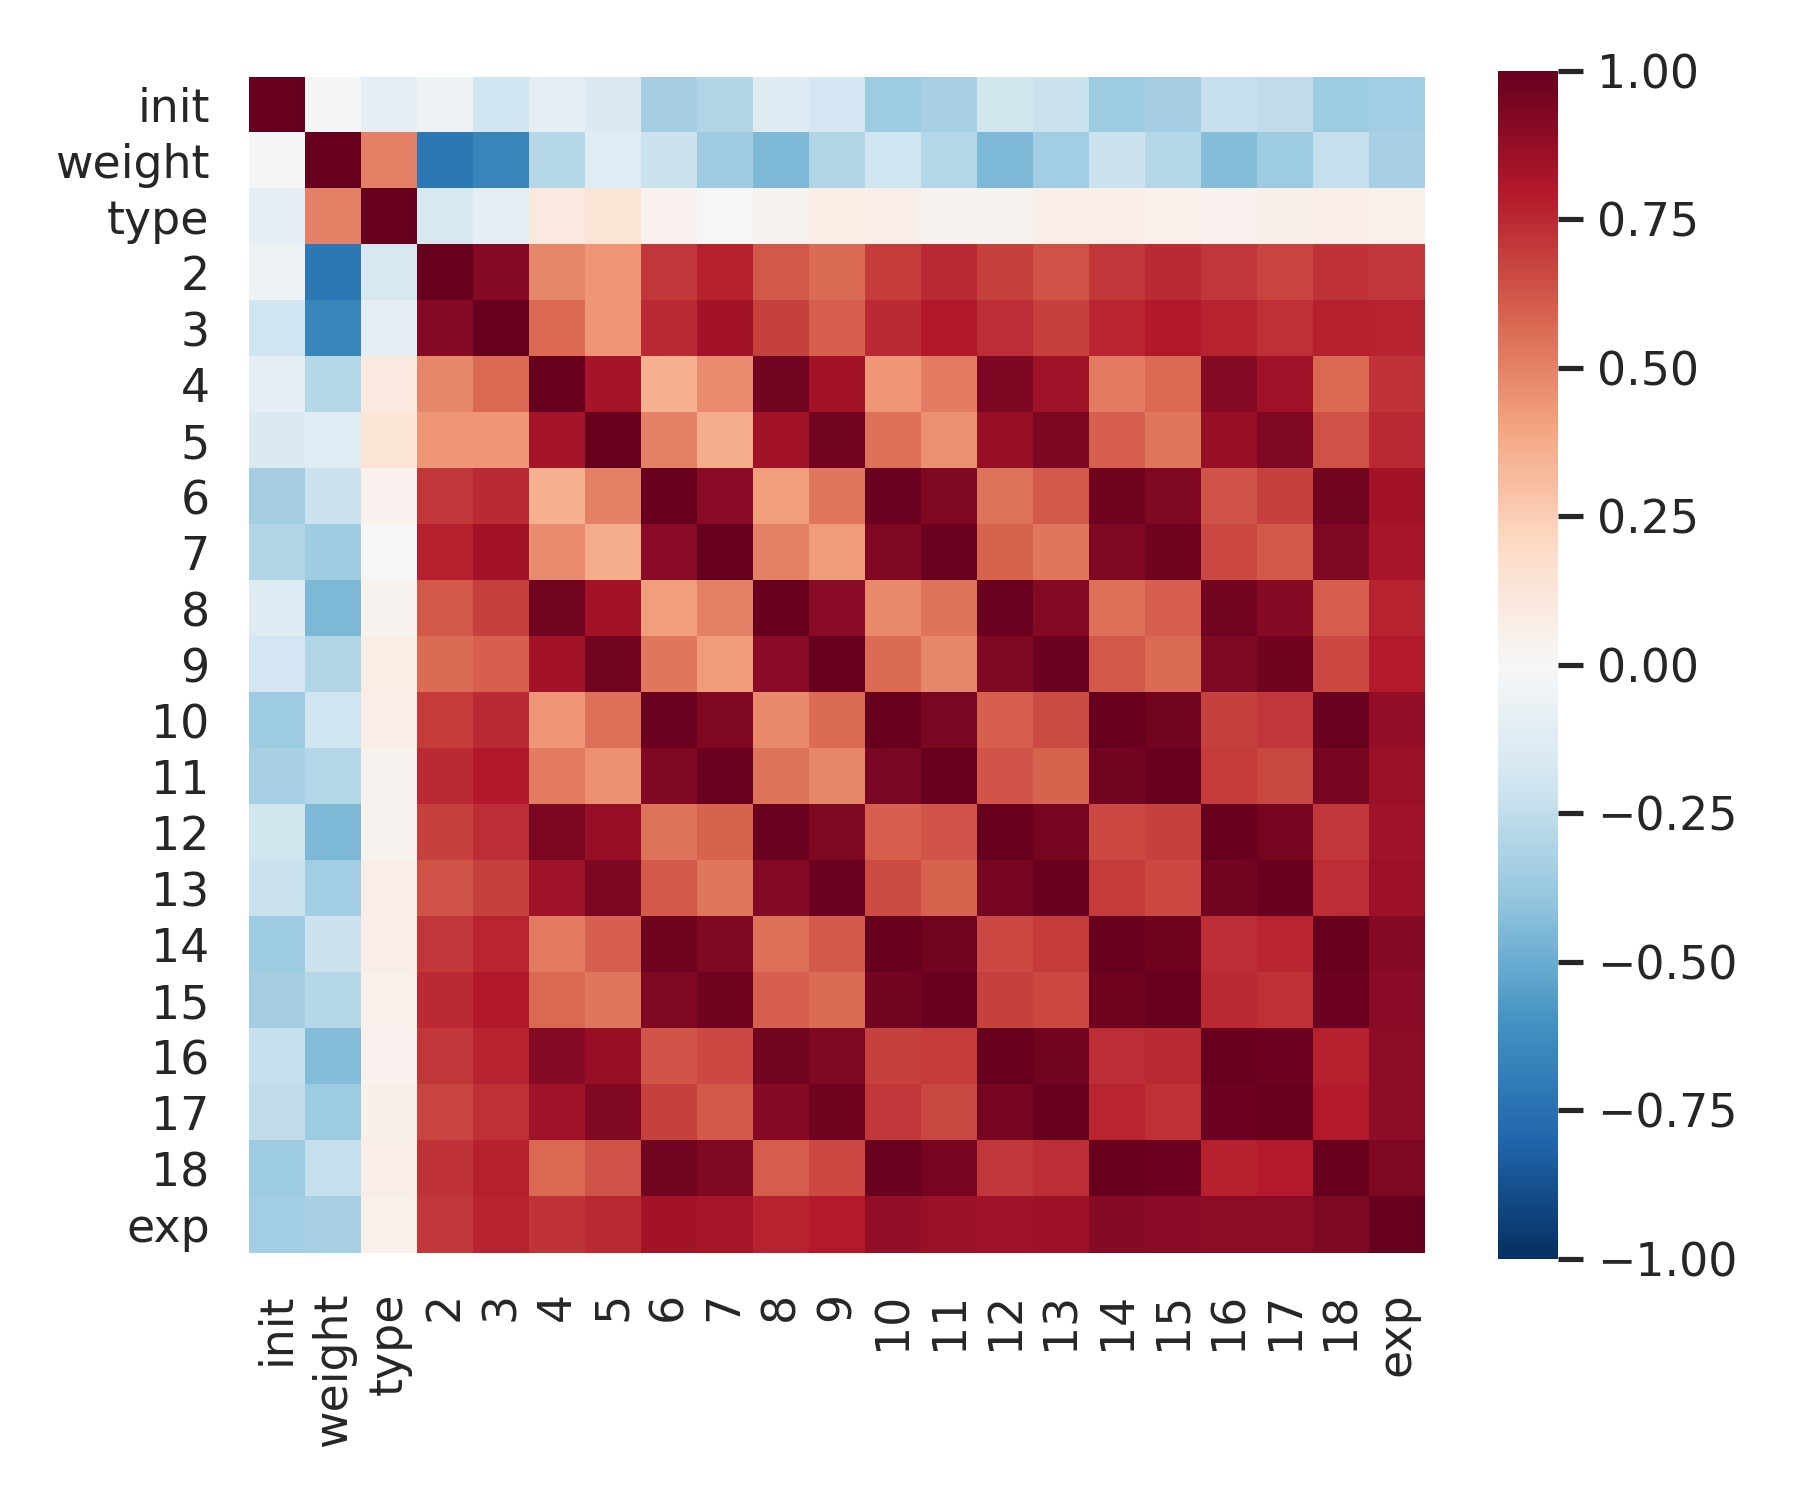
\includegraphics[width=\linewidth]{img/corr_mat_low}
    \caption{\texttt{weight} $< 1.5$.}
  \end{subfigure}
  \begin{subfigure}{0.32\textwidth}
    \centering
    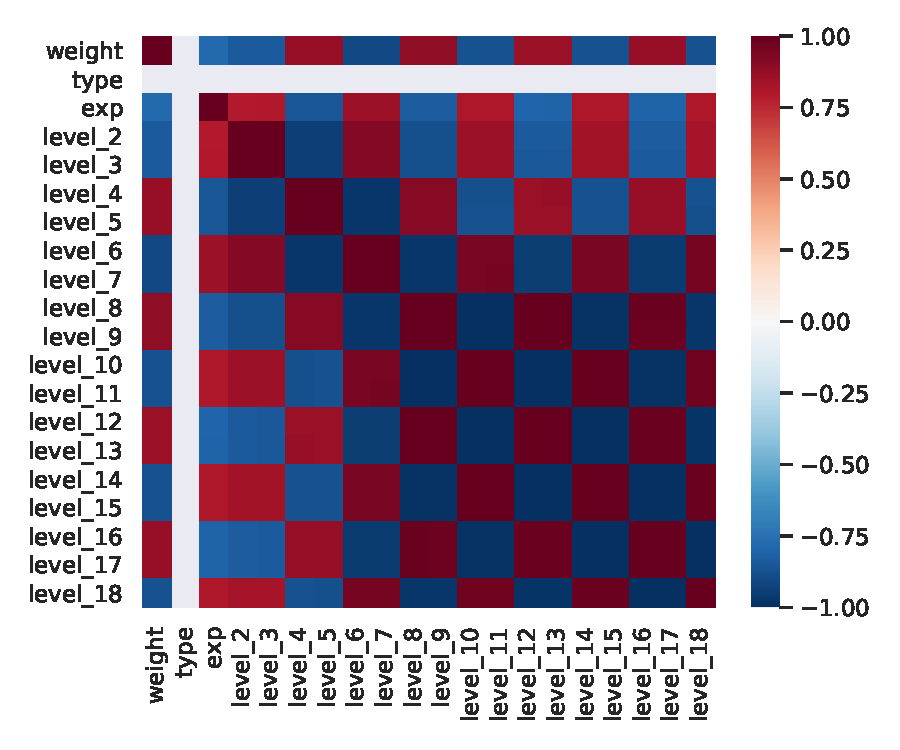
\includegraphics[width=\linewidth]{img/corr_mat_high}
    \caption{\texttt{weight} $\ge 1.5$.}
  \end{subfigure}
  \caption{Correlation matrices of the variables.}
  \label{fig:lumps:corr}
\end{figure}


\subsubsection{Principal Components Analysis}

We perform the Principal Components Analysis (\pca) of the truncation levels to study their properties and their distribution: it encodes the linear variance of the samples by projecting the distribution onto a new system of coordinates trying to maximise such variance in each new axis.
This approach may be interesting both as exploratory analysis and for further directions: we may want to generalise the algorithm to an arbitrary number of truncation levels (and we may want to skip some values).
The \pca would then give a solution to always have input of the same size while keeping as much information as possible.

We first study all principal components using the Singular Value Decomposition (\svd) of the matrix holding samples over the rows and the truncation levels over the columns (it is a rectangular matrix and as such cannot be strictly diagonalised to perform spectral analysis).
In \Cref{fig:lumps:svd} we show the variance explained by each principal component of the matrix (i.e.\ the fraction of variance of the total set retained by considering only the selected component).

\begin{figure}[htbp]
  \centering
  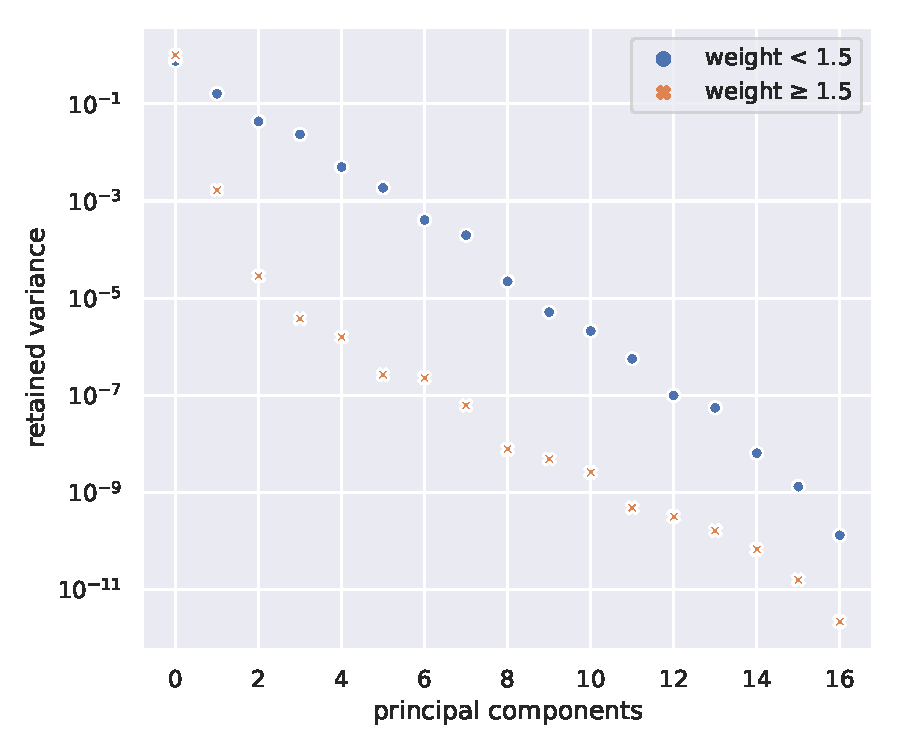
\includegraphics[width=0.6\textwidth]{img/svd}
  \caption{Variance explained by the principal components of the truncation levels (log scale).}
  \label{fig:lumps:svd}
\end{figure}

The analysis was performed splitting the values of the truncation levels over ranges of the \texttt{weight} variable.
The two folds have then been separately scaled: values of \texttt{weight} $< 1.5$ have been standardised (i.e.\ centered and scaled by their standard deviation), while the remaining values have been robustly scaled (i.e.\ centered and scaled by their interquartile) against the outliers present.
The result shows that for lower weights the first two principal components account for more than \SI{90}{\percent} of the total variance of the values, while for larger weights almost \SI{100}{\percent} of the variance is explained by the first component (in fact the \SI{99}{\percent} of the variance can be reached using 4 components for \texttt{weight} $< 1.5$, while the first component for \texttt{weight} $\ge 1.5$ already contains \SI{99.8}{\percent} of the total variance).
This is a reflection the distribution of the variables in the dataset: larger weights contain a very large amount of outliers and have larger variance with respect to lower weights.
It is then enough to project the values of the truncation levels over the line which contains most of the deviation to reproduce a meaningful distribution.


\subsubsection{K-Means Clustering}

Finally we perform an unsupervised clustering analysis of the truncation levels.
The main idea is to infer a structure in the data which may be able to ``automatically'' reproduce the labels (i.e.\ the \texttt{exp} column) without regression.
In other words we study the distribution of the truncation levels and fit it in 3 clusters representing the 3 integer values of the labels.\footnotemark{}
\footnotetext{%
  This analysis is strongly related to the finite number of unique values of the label in the dataset (for instance, the number of clusters has been chosen to match the number of unique values of \texttt{exp}).
  It might not be possible to repeat or generalise this procedure to other datasets.
}
In the ideal scenario there should be a 1:1 relation between the labels of the cluster centroids and the labels in the \texttt{exp} variable.
Unfortunately the cluster analysis of the truncation levels over the entire dataset highlighted no particular structure in the data and turned out inconclusive.

We then performed the same analysis splitting the dataset in different ranges of the \texttt{weight} variable, standardising the data for \texttt{weight} $< 1.5$ and robustly scaling (i.e.\ scaling according the interquartile range) samples for which \texttt{weight} $\ge 1.5$.
In \Cref{fig:lumps:kmeans} we used the principal components of the truncation levels to plot the distribution of the clusters and the \texttt{exp} labels.

\begin{figure}[htbp]
  \centering
  \begin{subfigure}{0.45\textwidth}
    \centering
    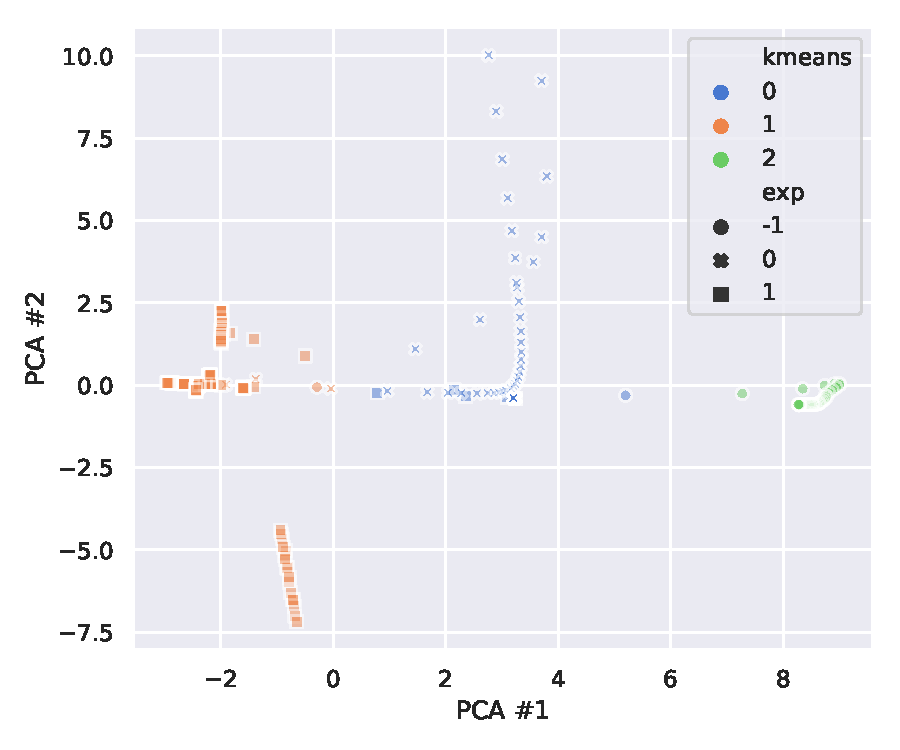
\includegraphics[width=\linewidth]{img/kmeans_low}
    \caption{\texttt{weight} $< 1.5$.}
  \end{subfigure}
  \begin{subfigure}{0.45\textwidth}
    \centering
    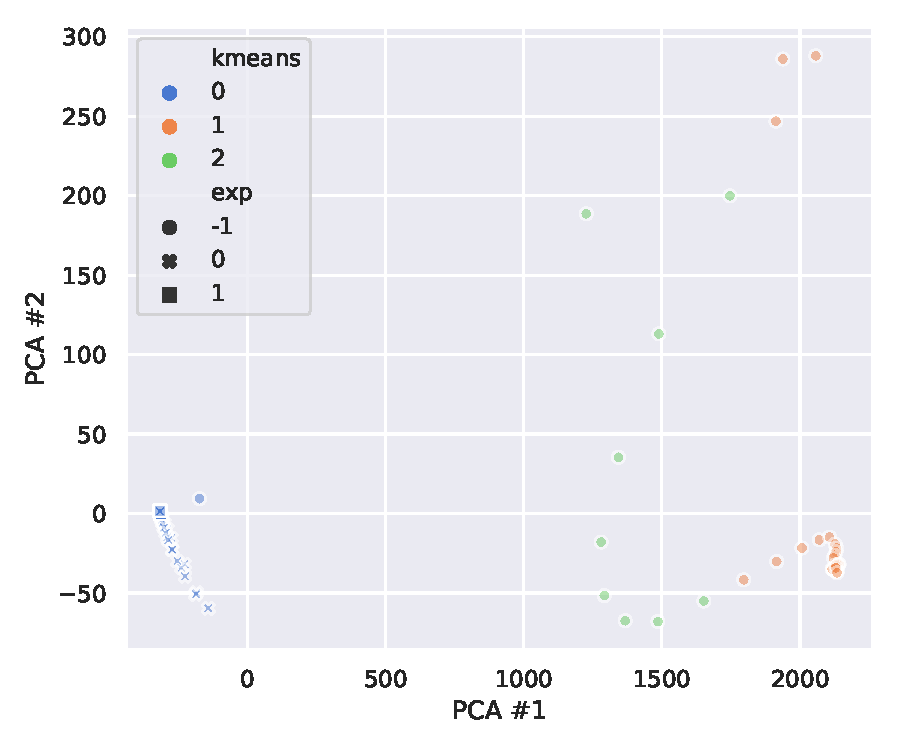
\includegraphics[width=\linewidth]{img/kmeans_high}
    \caption{\texttt{weight} $\ge 1.5$.}
  \end{subfigure}
  \caption{K-Means clusters and \texttt{exp} labels plotted using the principal
  components for visualisation purposes.}
  \label{fig:lumps:kmeans}
\end{figure}

\begin{table}[htbp]
  \centering
  %\resizebox{\textwidth}{!}{%
  \begin{tabular}{@{}ccc@{}}
  \toprule
               & \multicolumn{2}{c}{\textbf{K-Means}} \\
  \texttt{exp} & $\mu$             & $\sigma$        \\ \midrule
  -1           & 1.9               & 0.4             \\
  0            & 0.1               & 0.3             \\
  1            & 0.98              & 0.14            \\ \bottomrule
  \end{tabular}%
  %}
  \caption{Average cluster label for \texttt{weight} $< 1.5$ ($\mu$ is the average value and $\sigma$ its standard deviation).}
  \label{tab:lumps:kmeans}
\end{table}

As we can see, recognising a structure is challenging when \texttt{weight} $\ge 1.5$ and in fact different \texttt{exp} (or ``extrapolation'') labels generally belong to different clusters.
However the case \texttt{weight} $< 1.5$ seems to be more accurate and shows that in general we can recognise a structure in the data.
This is summarised in \Cref{tab:lumps:kmeans} where we show that there is a distinguishable relation between the extrapolation column and the average cluster label in the group
when \texttt{weight} $< 1.5$, while in general there is a superposition of
labels when \texttt{weight} $\ge 1.5$ (specifically it seems that there are only 2 recognisable clusters since both \texttt{exp} $= 0$ and \texttt{exp} $= 1$ share identically the same cluster label).


\subsection{Statistical Inference}

After the \eda we proceed with the study of statistical inference using linear models on the data.
The purpose of the analysis is to better understand the contribution of each variable to the predictions and study the relations among different features.
In the following we will be mainly interested in highlighting the properties of the dataset, while we only marginally mention the predictive ability of the linear model.
We use a simple linear regression without regularisation (using the class \texttt{LinearRegression} in \texttt{Scikit-learn}).

In order to avoid biasing the results, we split the dataset into a training set made of \SI{80}{\percent} of the samples and a development set made of the remaining entries.
The division has been made using the unique values of the \texttt{solutions} column: we first select what solutions to insert in the training and development folds and then assign the corresponding samples to the different sets.
This has the results of keeping similar distributions inside the same set and facilitate the training.\footnotemark{}
\footnotetext{%
  This is again deeply connected with the particular dataset we are using: it might not be possible to generalise such procedure, even though in this case it may help improving the results.
}
We also remove the case \texttt{solutions} $= 0$ (i.e.\ the first entry of the original untidied dataset) because its structure might spoil the generalisation properties since its values are too correlated with the output.

After training the linear model on the training fold, we analyse the outcome on the development set.
With 118 degrees of freedom (\dof) we reach a mean squared error (\mse) of \num{0.16} with a \SI{95}{\percent} confidence interval (\ci) $[0.10, 0.23]$ and a \emph{coefficient of determination} \rr of \num{0.68}.\footnotemark{}
\footnotetext{%
  The coefficient of determination is a measure of the fraction of the variance of the data explained by the model (sometimes it is referred to as \emph{fraction of variance explained}).
  Its definition is however different from the coefficient of correlation $\rho$ also used in statistics.
  In fact, let
  \begin{equation*}
    S_{res}(y, \hat{y}) = \finitesum{i}{1}{N} (y_i - \hat{y}_i)^2,
    \qquad
    S_{tot}(y) = \finitesum{i}{1}{N} (y_i - \bar{y})^2,
  \end{equation*}
  where $N$ is the number of samples, $y$ are the ``experimental'' data, $\bar{y}$ is the sample average of them, and $\hat{y}$ are the predicted data.
  Then the coefficient of determination is defined as:
  \begin{equation*}
    \rr = 1 - \frac{S_{res}(y, \hat{y})}{S_{tot}(y)}
        = 1 - \textrm{FVU},
  \end{equation*}
  where FVU stands for \emph{Fraction of Variance Unexplained}, that is the amount of variance of the data which the model cannot account for.
  A perfect predictor would have $\rr = 1$ (i.e.\ it is capable of reproducing the full variance of the data), while a poor model can have negative values.
}
The interesting part of the analysis is however the \emph{ANalysis Of VAriance} (\anova) of the coefficients summarised in \Cref{tab:lumps:anova} (we do not report the \ci for brevity, since in this case the p-value holds more than enough information).
As we can see the large variance associated with the values of each variable led to a very precise determination of the coefficients (as feared, even too precise).
As a consequence, the p-value associated to the observation of more extreme values than those computed here is vanishing for almost all coefficients.
The \texttt{type} variable however has a different behaviour: according to its associated p-value we might consider removing it from the input features.
However such feature, even though irrelevant for the fit, plays an important role when distinguishing higher and lower weights.
We will therefore keep it in the input features to help the algorithms in training (especially the decision trees).\footnotemark{}
\footnotetext{%
  We also repeated the same statistical inference removing the \texttt{type} variable and, as expected, the \anova did not show any difference: all p-values are vanishing in any case.
  However the predictions suffered from the missing variable.
}

\begin{table}[htbp]
  \centering
  %\resizebox{\textwidth}{!}{%
  \begin{tabular}{@{}ccccc@{}}
  \toprule
                     & \textbf{coefficient}        & \textbf{standard error} & \textbf{Student's t} & \textbf{p-value} ($t_{obs} \ge \abs{t}$)  \\
  \midrule
  \texttt{weight}    & 0.109                       & 0.015                   & 7                    & 0.0                                       \\
  \texttt{type}      & 0.03                        & 0.05                    & 0.6                  & 0.5                                       \\
  \texttt{level 2}   & -0.067                      & 0.007                   & -9                   & 0.0                                       \\
  \texttt{level 3}   & 0.135                       & 0.007                   & 20                   & 0.0                                       \\
  \texttt{level 4}   & -0.2955                     & 0.0014                  & $-2 \times 10^2$     & 0.0                                       \\
  \texttt{level 5}   & 0.4161                      & 0.0014                  & $3 \times 10^3$      & 0.0                                       \\
  \texttt{level 6}   & $-2904 \times 10^{-4}$      & $3 \times 10^{-4}$      & $-9 \times 10^3$     & 0.0                                       \\
  \texttt{level 7}   & $4527 \times 10^{-4}$       & $3 \times 10^{-4}$      & $1.5 \times 10^3$    & 0.0                                       \\
  \texttt{level 8}   & $-41345 \times 10^{-5}$     & $6 \times 10^{-5}$      & $-7 \times 10^3$     & 0.0                                       \\
  \texttt{level 9}   & $57675 \times 10^{-5}$      & $6 \times 10^{-5}$      & $1.0 \times 10^3$    & 0.0                                       \\
  \texttt{level 10}  & $-31909 \times 10^{-5}$     & $1.3 \times 10^{-5}$    & $-2 \times 10^4$     & 0.0                                       \\
  \texttt{level 11}  & $43550 \times 10^{-5}$      & $1.3 \times 10^{-5}$    & $3 \times 10^4$      & 0.0                                       \\
  \texttt{level 12}  & $-191313 \times 10^{-6}$    & $3 \times 10^{-6}$      & $-5 \times 10^4$     & 0.0                                       \\
  \texttt{level 13}  & $249714 \times 10^{-6}$     & $3 \times 10^{-6}$      & $6 \times 10^4$      & 0.0                                       \\
  \texttt{level 14}  & $-602220 \times 10^{-7}$    & $8 \times 10^{-7}$      & $-3 \times 10^4$     & 0.0                                       \\
  \texttt{level 15}  & $808300 \times 10^{-7}$     & $8 \times 10^{-7}$      & $4 \times 10^4$      & 0.0                                       \\
  \texttt{level 16}  & $59010 \times 10^{-7}$      & $2 \times 10^{-7}$      & $-5 \times 10^3$     & 0.0                                       \\
  \texttt{level 17}  & $103750 \times 10^{-7}$     & $2 \times 10^{-7}$      & $8 \times 10^3$      & 0.0                                       \\
  \texttt{level 18}  & $43700 \times 10^{-8}$      & $7 \times 10^{-8}$      & $4 \times 10^2$      & 0.0                                       \\
  \bottomrule
  \end{tabular}%
  %}
  \caption{Analysis of the coefficients of the linear model.}
  \label{tab:lumps:anova}
\end{table}


\subsection{Model Dependent Machine Learning Analysis}

\subsubsection{Validation and Evaluation Strategy}

As for the previous section, in the \ml analysis we use the tidy dataset without the samples corresponding to \texttt{solutions} $= 0$ to try and retain as much generalisation capability as possible.
We also keep samples corresponding to the same values of \texttt{solutions} in the same set to balance the distribution of the samples as before.
Since the number of samples is small, we will use a single validation set to evaluate the algorithms and perform the optimisation of the hyperparameters.
However, before choosing the validation strategy, we first split the dataset in two folds: the first holds \SI{90}{\percent} of the samples and will be used for training and validation, while the remaining \SI{10}{\percent} will be used for testing.

\begin{figure}[htbp]
  \centering
  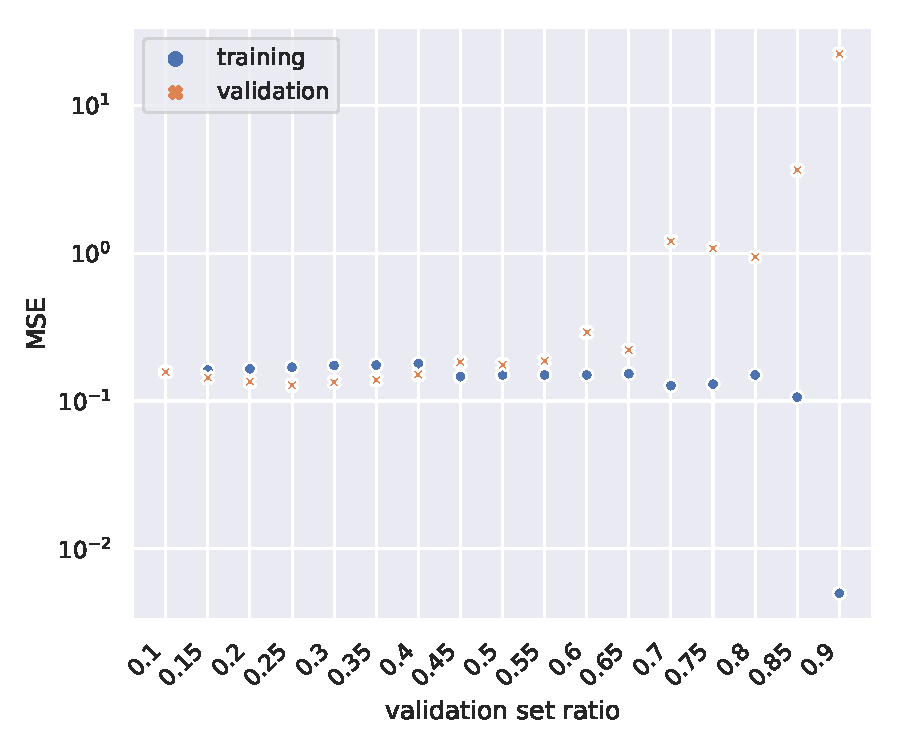
\includegraphics[width=0.6\textwidth]{img/valsize_errors}
  \caption{\mse in training and validation for different validation ratios.}
  \label{fig:lumps:validation_size}
\end{figure}

We then choose the size of the validation set to be around \SI{10}{\percent} of the total training set as it is typical for datasets of this dimension where most of the samples should be assigned to training.
Another motivation for the choice is to try to minimise the error (\mse) made when fitting a linear regression on decreasing size of the set effectively used for training, after removing the validation split: this may clearly not work for anything different from a linear model, but it is however a good starting point.
In \Cref{fig:lumps:validation_size} we show training and validation \mse for different sizes of the validation set (with respect to the total training set).
In order to keep a reasonable amount of samples in the training split and to contain the validation \mse as much as possible, we finally take the already mentioned \SI{10}{\percent} of the unique \texttt{solutions} in the validation set.

\begin{table}[htbp]
\centering
\begin{tabular}{@{}ccc@{}}
\toprule
           & \multicolumn{2}{c}{\textbf{total dataset}} \\
           & \textit{samples}    & \textit{fraction}    \\
\midrule
training   & 584                 & 80\%                 \\
validation & 68                  & 9\%                  \\
test       & 80                  & 11\%                 \\
\bottomrule
\end{tabular}
\caption{Summary of the train/validation/test splits.}
\label{tab:lumps:splits}
\end{table}

In \Cref{tab:lumps:splits} we give a schematic summary of the final choice for training, validation and test sets after assigning the samples corresponding to the chosen \texttt{solutions} in each fold. 


\subsubsection{Training}

For the \ml analysis we first scale the truncation levels using a robust scaler (the \texttt{RobustScaler} in \texttt{Scikit-learn}).
We then include also the variables \texttt{weight} and \texttt{type} into the input features.
In \Cref{tab:lumps:preds} we summarise the predictions of different algorithms after optimisation (we use Bayes optimisation techniques implemented in \texttt{Scikit-optimize} to look for the best hyperparameters): \emph{LR} refers to linear regression (with $\ell_2$ regularisation), \emph{l-SVR} is the linear implementation of support vector machines for regression, \emph{r-SVR} uses a \emph{kernel trick} (with a Gaussian function, or \emph{radial} function) for support vectors, \emph{RF} are random forests of decision trees, \emph{GBDT} are gradient boosted decision trees, and finally \emph{ANN} refers to artificial neural networks.\footnotemark{}
\footnotetext{%
  This model is made of 4 hidden layers with \numlist{30;20;20;10} units each and ReLU activation.
  Batch normalisation (with momentum \num{0.99}) follows each layer.
  Dropout layers (with rate \num{0.01}) are used only after the first two layers.
  The output is made of a single unit without activation function.
  We use the \mse as loss function.
  Gradient descent is computed using the \emph{Adam} optimiser with default parameters and a mini batch size of 32.
  Training is early stopped after 5000 epochs without loss improvement on the validation set and the learning rate (initially set at \num{0.01}) is reduced by a factor \num{0.3} after 2500 epochs without loss improvement.
  While it is in general important to keep track of the models used, the architecture of the aggregate analysis is substantially different, thus making this model not particularly useful.
}

\begin{table}[htbp]
  \centering
  %\resizebox{\textwidth}{!}{%
  \begin{tabular}{@{}ccccc@{}}
  \toprule
                            & \textbf{MSE} & \textbf{95\% C.I.}  & \textbf{MAE} & $r^2$ \\
  \midrule
  \emph{LR ($\ell_2$ reg.)} & 0.16         & (0.07, 0.25)        & 0.3          & 0.68        \\
  \emph{l-SVR}              & 2.4          & (-0.2, 5.1)         & 0.5          & -3.77       \\
  \emph{r-SVR}              & 0.030        & (0.005, 0.046)      & 0.08         & 0.95        \\
  \emph{RF}                 & 0.011        & (-0.003, 0.025)     & 0.04         & 0.98        \\
  \emph{GBDT}               & 0.00085      & (-0.00015, 0.00185) & 0.016        & 1.00        \\
  \emph{ANN}                & 0.00004      & (0.0002, 0.0005)    & 0.005        & 1.00        \\
  \bottomrule
  \end{tabular}%
  %}
  \caption{%
    Summary of the predictions on the test set.
    The number of \dof\ has been taken to be constant for alla algorithms ($80 - 21 = 59$) as in the linear model for a direct comparison.
  }
  \label{tab:lumps:preds}
\end{table}

As we can see both \emph{GBDT} and \emph{ANN} are able to deliver consistency and precision in the predictions on the test set.
As shown in \Cref{fig:lumps:best} both algorithms perform extremely well on the test set as also the histograms of the residuals in \Cref{fig:lumps:hist} are able to show.

\begin{figure}[htbp]
  \centering
  \begin{subfigure}{0.45\textwidth}
    \centering
    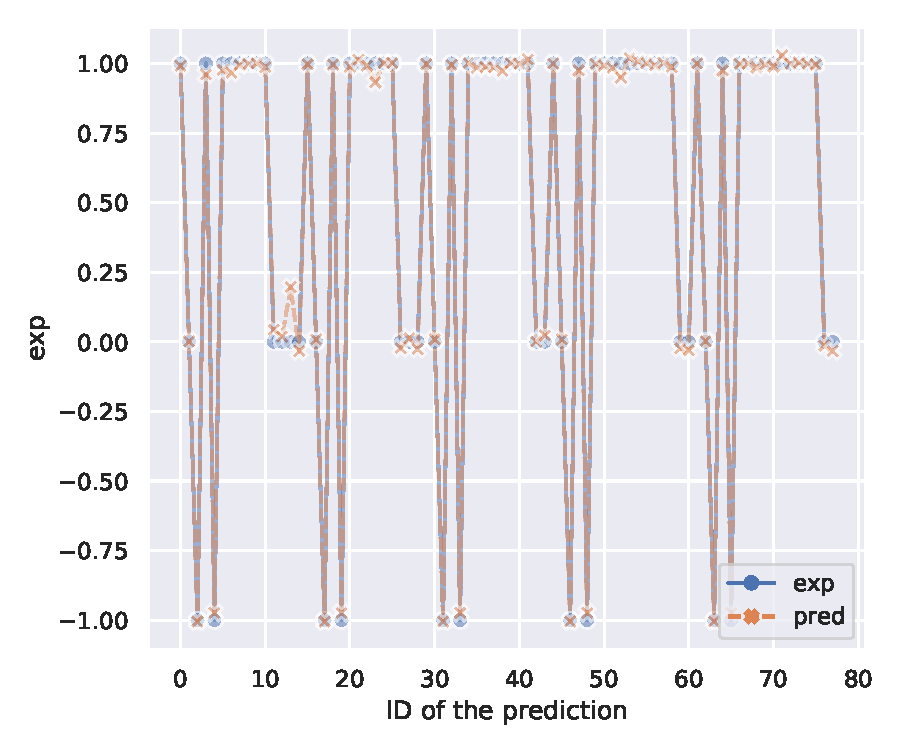
\includegraphics[width=\linewidth]{img/gbdt_lgbmregressor_test_lineplot}
    \caption{\emph{GBDT} predictions and ground truth.}
  \end{subfigure}
  \begin{subfigure}{0.45\textwidth}
    \centering
    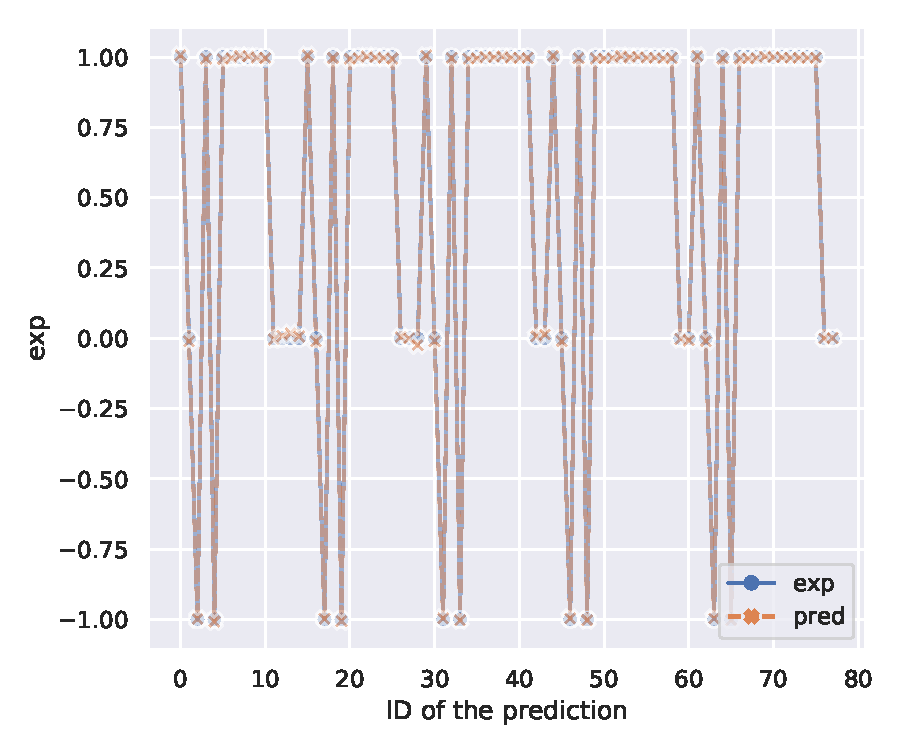
\includegraphics[width=\linewidth]{img/ann_model_test_lineplot}
    \caption{\emph{ANN} predictions and ground truth.}
  \end{subfigure}
  \caption{Predictions and true values for the best algorithms.}
  \label{fig:lumps:best}
\end{figure}

\begin{figure}[htbp]
  \centering
  \begin{subfigure}{0.45\textwidth}
    \centering
    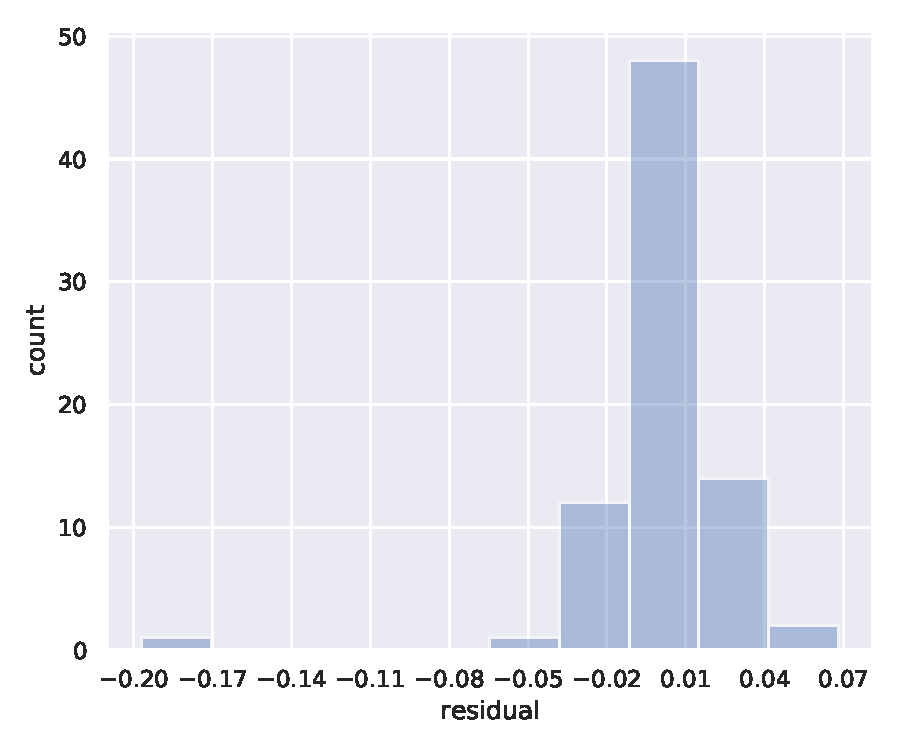
\includegraphics[width=\linewidth]{img/gbdt_lgbmregressor_test_histogram}
    \caption{\emph{GBDT} residuals.}
  \end{subfigure}
  \begin{subfigure}{0.45\textwidth}
    \centering
    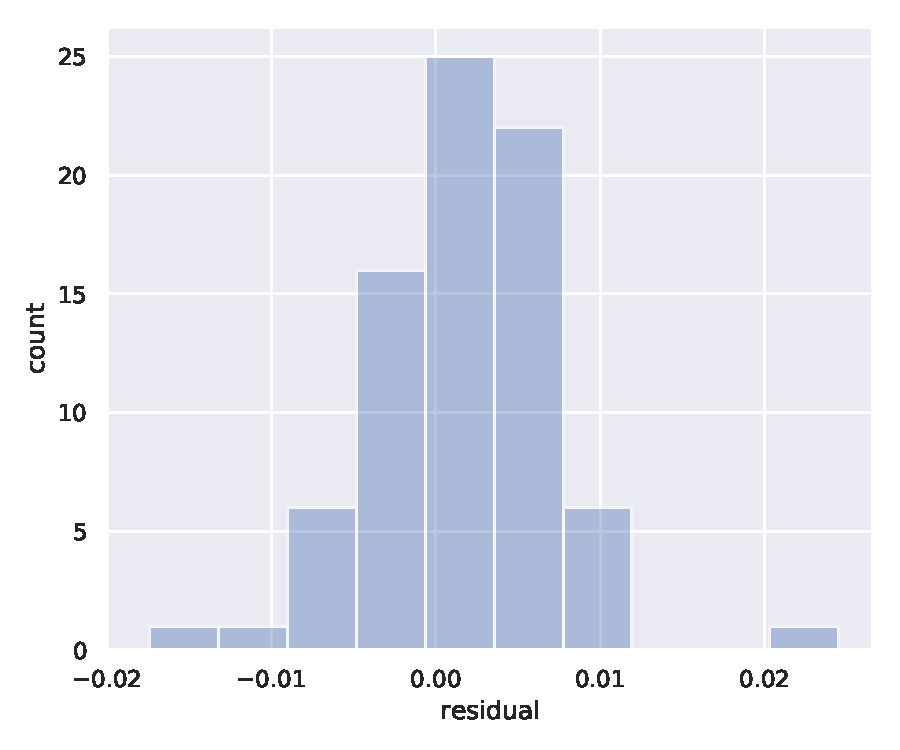
\includegraphics[width=\linewidth]{img/ann_model_test_histogram}
    \caption{\emph{ANN} residual.}
  \end{subfigure}
  \caption{Histogram of the residuals.}
  \label{fig:lumps:hist}
\end{figure}

Given the results of both algorithms we may therefore be interested in seeing the generalisation abilities and the versatility shown by the ANNs on other datasets.
While they both perform well, the ANN might in fact behave better when changing the underlying dataset.
As a matter of fact, though extremely good when the training and real world sets have the same distributions, decision trees suffer a lot under small changes in the data: their good performance may therefore be due to the particular range of the label \texttt{exp}.
For generalisation purposes we will therefore focus on the \emph{ANN}.


\subsubsection{Analysis of the Features}

After training the algorithms, we focus on studying the outcome of the decision trees (namely the \emph{RF} and the \emph{GBDT}).
We are interested in better understanding the contributions of each variable to the results through the study of the variable ranking (i.e.\ the feature importances) and the Shapley values.
In \Cref{tab:lumps:hyp} we show the choices of the hyperparameters used for training the decision trees algorithms and which will influence to following analysis.
As we could have imagined, \emph{GBDT}s prefer a larger number of boosting rounds made of small trees, while \emph{RF} prefer a smaller number of fully grown trees.
The relative weight of each sample in the tree changes in both implementations of the decision trees and is definitely more relevant when the trees are smaller (i.e.\ in the \emph{GBDT}).
Both $\ell_1$ (\texttt{reg\_alpha}) and $\ell_2$ (\texttt{reg\_lambda}) regularisation have been used to produce the predictions.

\begin{table}[htbp]
  \centering
  \begin{tabular}{@{}lrr@{}}
      \toprule
      \textbf{hyperparameters}    & \textbf{RF} & \textbf{GBDT} \\
      \midrule
      \texttt{num\_leaves}        & 70          & 10            \\
      \texttt{max\_depth} 	  & 500         & 25            \\
      \texttt{learning\_rate}     & ---         & 0.1           \\
      \texttt{n\_estimators} 	  & 50          & 1590          \\
      \texttt{subsample} 	  & 0.99        & 0.66          \\
      \texttt{colsample\_bytree}  & 1.00        & 1.00          \\ \texttt{min\_child\_weight} & $10^{-6}$   & $10^{-3}$     \\
      \texttt{reg\_alpha} 	  & 0.1         & 1.0           \\
      \texttt{reg\_lambda}        & 0.12        & 1.0           \\
      \bottomrule
  \end{tabular}
  \caption{Hyperparameters used by \emph{RF} and \emph{GBDT}.}
  \label{tab:lumps:hyp}
\end{table}

The importance of the features is a key property of the decision trees and visually summarises the impact that each feature has on the final prediction: variables with higher importance can be found in the first branches of the trees because they are responsible for the main choices of the algorithm, while more negligible features provide the necessary refinement.
The Shapley values are somewhat related and derive from a game theoretic approach to the decision trees: these values encode how a certain feature is influencing the final result, whether by dragging its value with respect to average of the predictions or by pushing it beyond it.
In other words, feature importances show how much (as a percentage of the final prediction) a variable is relevant for the algorithm and the Shapley values show if there are variables which tend to drive the results towards a
particular value.

\begin{figure}[htbp]
  \centering
  \begin{subfigure}{0.45\textwidth}
    \centering
    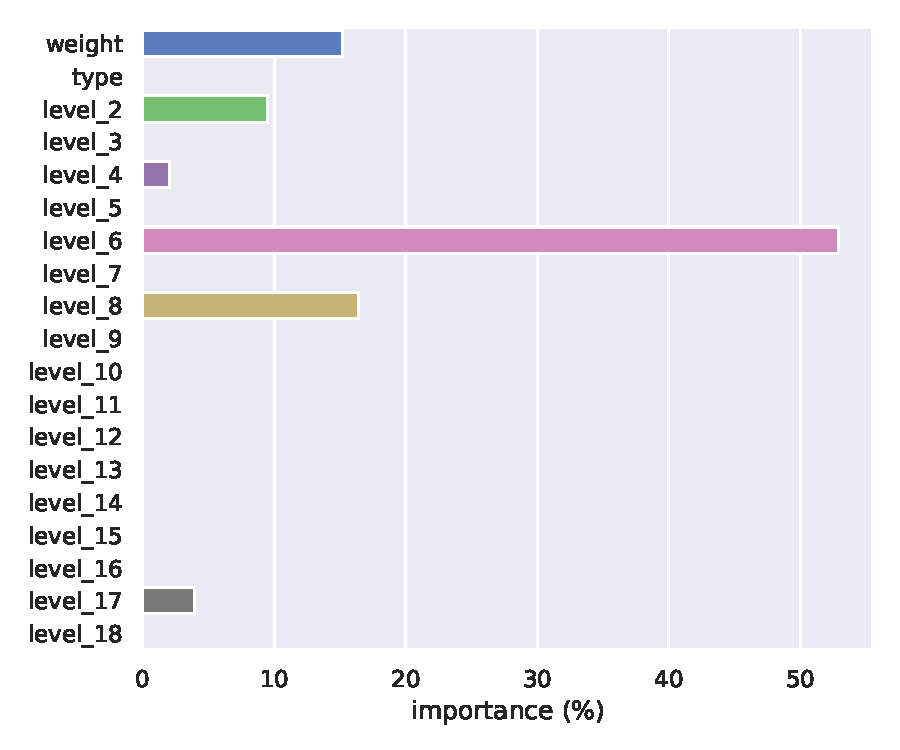
\includegraphics[width=\linewidth]{img/rnd_for_rank}
    \caption{Variable ranking.}
  \end{subfigure}
  \begin{subfigure}{0.45\textwidth}
    \centering
    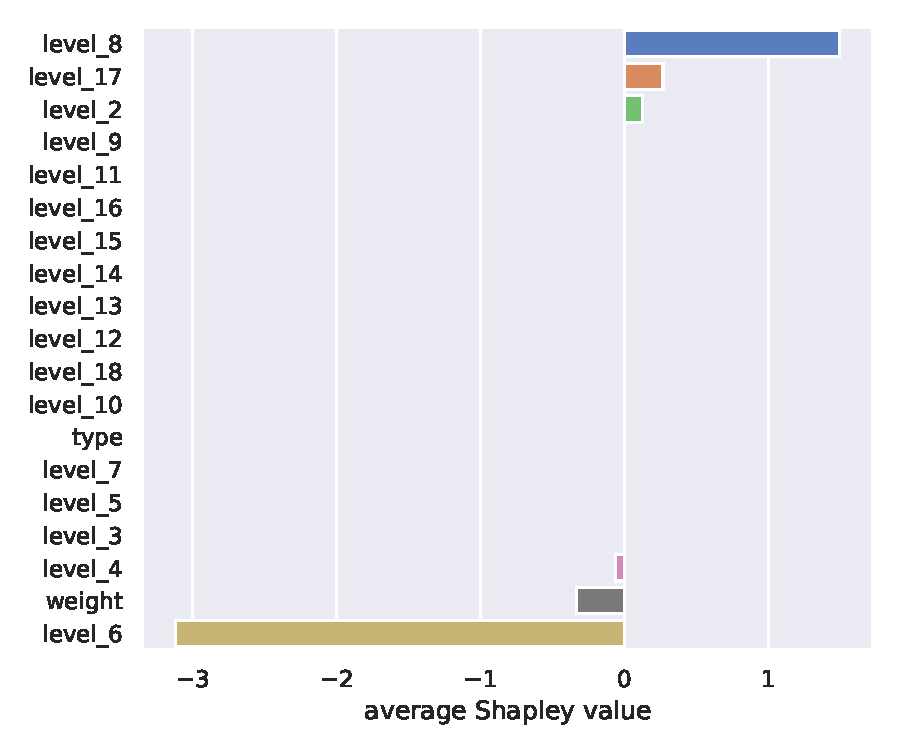
\includegraphics[width=\linewidth]{img/rnd_for_shap}
    \caption{Shapley values.}
  \end{subfigure}
  \caption{Feature importances and Shapley values of the \emph{RF}.}
  \label{fig:lumps:rnd_for}
\end{figure}

In \Cref{fig:lumps:rnd_for} we show the variable ranking and the Shapley values for the \emph{RF} algorithm.
The first plot shows that RF rely on a particular truncation level (\texttt{level\_6} to be specific) to produce the predictions, while other features contribute in a less relevant manner.
The average Shapley values (second plot) show that most features give a comparable contribution to the prediction, exception made for the mass truncation at \texttt{level\_6} which seems to drive the final result in a more direct way (according to \Cref{fig:lumps:counts} they are among the highly unbalanced values, which may be a reason for such behaviour).

\begin{figure}[htbp]
  \centering
  \begin{subfigure}{0.45\textwidth}
    \centering
    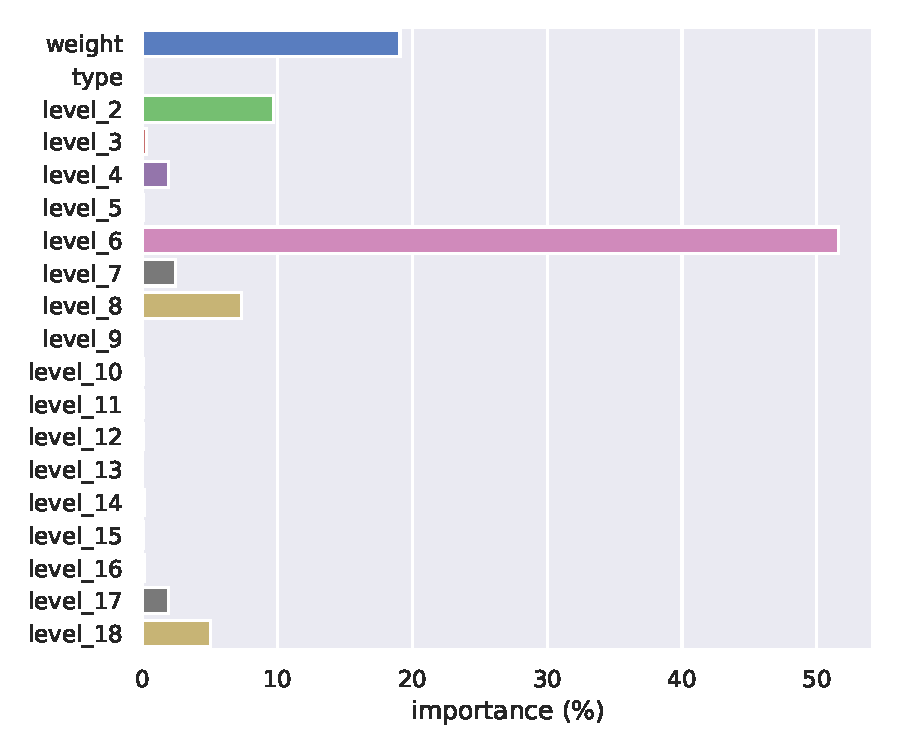
\includegraphics[width=\linewidth]{img/grd_bst_rank}
    \caption{Variable ranking.}
  \end{subfigure}
  \begin{subfigure}{0.45\textwidth}
    \centering
    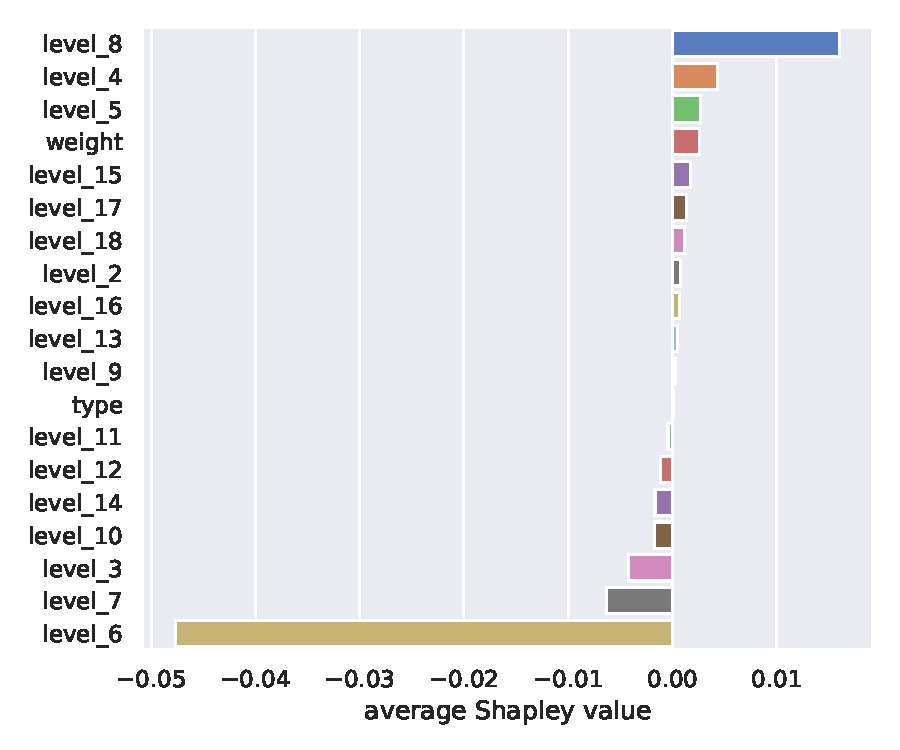
\includegraphics[width=\linewidth]{img/grd_bst_shap}
    \caption{Shapley values.}
  \end{subfigure}
  \caption{Feature importances and Shapley values of the \emph{GBDT}s.}
  \label{fig:lumps:grd_bst}
\end{figure}

In \Cref{fig:lumps:grd_bst} we finally show the same plot for the \emph{GBDT}s.
Differently from the \emph{RF}, \emph{GBDT}s seem to rely almost entirely on the 6th truncation level and \texttt{weight} discrimination of the samples.
In both cases the algorithms seem to ignore almost completely the categorical variable \texttt{type} (possibly it could have been removed but the corresponding Shapley value shows that its relevance is so marginal that the result would not have changed).

We notice that the scale of the Shapley values is very different between \emph{RF} and \emph{GBDT}: this is due to the fact that in this case the boosting procedure may be more robust against the large variability of the dataset, showing that in the \emph{GBDT} case the trees are more balanced.
Ultimately this is also a consequence of the different order of magnitude of the \mse associated to \emph{RF} and \emph{GBDT}, the latter being almost an order of magnitude more precise than the former.

We also performed this type of analysis on \emph{GBDT} successively removing different subsamples of the features in the attempt to better understand the presence of one feature with a very high importance with respect to all others.
Results showed that whatever the subsample of features, the algorithm always chooses the 3rd to 5th level truncation level as most important: after guessing the behaviour based on the first few truncation levels, the algorithm finally predicts the label using one particular feature (\texttt{level\_6} in the case shown in the figures) and finally refines it using the last truncations levels.


\subsubsection{Double Lumps}

As a test of the generalisation ability of the algorithms, we perform predictions on double lumps solutions using the algorithms trained in the previous section (i.e.\ we do not perform again the optimisation and training procedure).
The dataset used is made of 20 entries with the same columns as the previous solutions.

Before making predictions, we scale the truncation levels using the same robust scaler we used in the previous section.
The predicted labels are then directly comparable with the real values.
In \Cref{tab:lumps:dlumps} we show the complete list of the predictions made on the double lumps.\footnotemark{}
\footnotetext{%
  Since the performance has been in general very poor, we removed the predictions using \emph{l-SVR} as model.
}
We kept \texttt{weight} and \texttt{type} to label each solution (we dropped the truncation levels for brevity).
Finally we pictorially show the predictions in \Cref{fig:lumps:dlump_preds}: as imagined, decision trees kept the prediction interval $[-1, 1]$ as the original dataset on which they were trained, while the \emph{ANN} extrapolated more.

\begin{figure}[htbp]
  \centering
  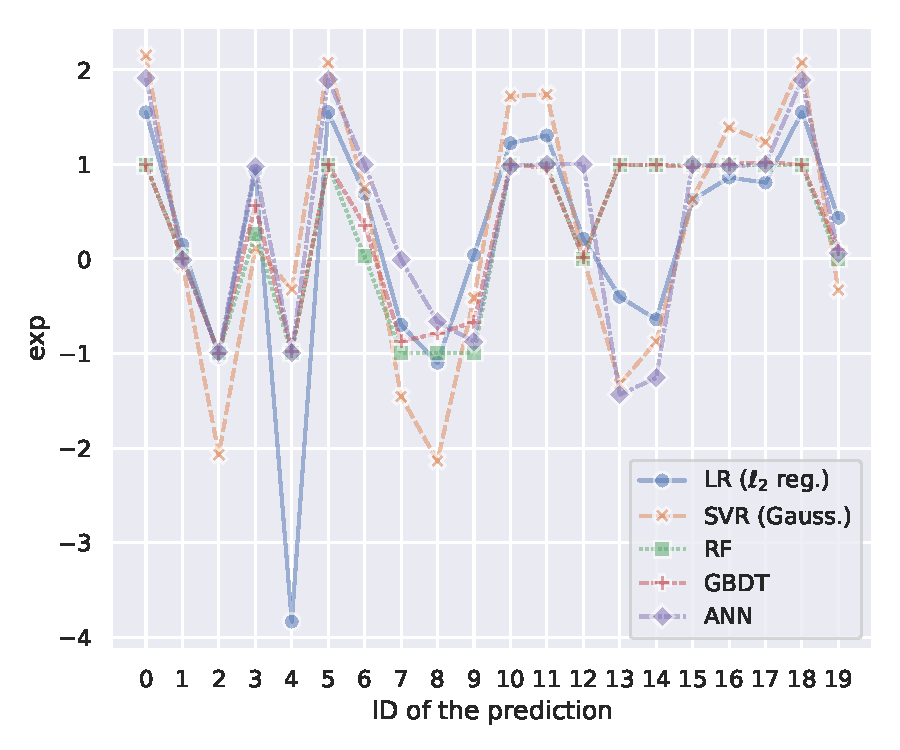
\includegraphics[width=0.6\textwidth]{img/dlumps_pred}
  \caption{Double lumps predictions.}
  \label{fig:lumps:dlump_preds}
\end{figure}

\begin{table}[htbp]
  \centering
  %\resizebox{\textwidth}{!}{%
  \begin{tabular}{@{}ccccccc@{}}
  \toprule
  \textbf{weight} & \textbf{type} & \textbf{exp (LR)} & \textbf{exp (r-SVR)} & \textbf{exp (RF)} & \textbf{exp (GBDT)} & \textbf{exp (ANN)} \\ \midrule
  0.000000        & 2             & 1.551467          & 2.153519             & 0.989096          & 0.994209            & 1.910616           \\
  0.000000        & 2             & 0.148665          & -0.054234            & 0.026711          & 0.008819            & -0.010774          \\
  1.000000        & 4             & -1.036330         & -2.071016            & -0.991434         & -0.998615           & -0.987881          \\
  4.000000        & 4             & 0.930320          & 0.114937             & 0.264700          & 0.563773            & 0.978944           \\
  9.000000        & 4             & -3.834771         & -0.322144            & -0.991861         & -0.974030           & -0.990880          \\
  0.000000        & 4             & 1.552892          & 2.075871             & 0.989096          & 0.995166            & 1.894776           \\
  0.027778        & 4             & 0.690183          & 0.749930             & 0.026711          & 0.358236            & 0.998884           \\
  0.111111        & 4             & -0.696637         & -1.455321            & -0.991434         & -0.869838           & -0.007325          \\
  0.250000        & 4             & -1.099292         & -2.137033            & -0.991434         & -0.787782           & -0.664277          \\
  0.444444        & 4             & 0.040714          & -0.412954            & -0.991434         & -0.667371           & -0.874694          \\
  0.694444        & 4             & 1.223861          & 1.721034             & 0.989096          & 1.000537            & 0.981812           \\
  1.000000        & 4             & 1.305418          & 1.741227             & 0.989096          & 0.962043            & 1.004753           \\
  1.361111        & 4             & 0.213720          & 0.014285             & 0.002803          & 0.019858            & 1.000996           \\
  1.777778        & 4             & -0.400493         & -1.323758            & 0.997782          & 0.996645            & -1.434201          \\
  2.250000        & 4             & -0.639370         & -0.874269            & 0.997782          & 0.995911            & -1.257340          \\
  2.777778        & 4             & 0.625367          & 0.635726             & 0.997782          & 0.971987            & 0.997438           \\
  3.361111        & 4             & 0.860903          & 1.392883             & 0.997782          & 1.002204            & 0.979112           \\
  4.000000        & 4             & 0.807342          & 1.234534             & 0.989096          & 1.023945            & 0.998200           \\
  0.000000        & 4             & 1.552892          & 2.075871             & 0.989096          & 0.995166            & 1.894776           \\
  2.250000        & 4             & 0.434775          & -0.329326            & 0.002803          & 0.101149            & 0.059882           \\ \bottomrule
  \end{tabular}%
  %}
  \caption{Predictions on the double lumps set.}
  \label{tab:lumps:dlumps}
\end{table}

We finally compare the results of the predictions of the double lumps with the extrapolated labels.
In order to keep only the most reliable results, we limit the predictions to \texttt{weight} $< 1.5$.
In \Cref{tab:lumps:double_metrics} we summarise the results which showed a good result for the \emph{r-SVR} algorithm with $\rr = 0.96$.

\begin{table}[htbp]
  \centering
  %\resizebox{\textwidth}{!}{%
  \begin{tabular}{@{}cccc@{}}
  \toprule
               & \mse & \mae & \rr   \\ \midrule
  \emph{LR}    & 0.3  & 0.5  & 0.85 \\
  \emph{r-SVR} & 0.10 & 0.3  & 0.96 \\
  \emph{RF}    & 0.6  & 0.7  & 0.72 \\
  \emph{GBDT}  & 0.6  & 0.7  & 0.72 \\
  \emph{ANN}   & 0.4  & 0.5  & 0.81 \\ \bottomrule
  \end{tabular}%
  %}
  \caption{Metrics computed on the double lumps with \texttt{weight} $< 1.5$.}
  \label{tab:lumps:double_metrics}
\end{table}


\subsection{Fourier Analysis and Signal Processing}


\subsubsection{Tidying the Dataset for the Analysis}

For the analysis we use the same dataset as in the rest of this section.
The main difference is how the \texttt{type} variable is considered: using the \texttt{get\_dummies} function in \texttt{pandas}, we convert the values to categorical labels.
The outcome of the operation is the conversion of the single \texttt{type} to two different columns in correspondence of the two different values taken by the entries (namely the new column \texttt{type\_2} has $1$ where \texttt{type} $= 2$ and $0$ elsewhere, and \texttt{type\_4} has $1$ where \texttt{type} $= 4$ and $0$ anywhere else).


\subsubsection{Training and Validation Strategy}

In this part of the analysis we change the approach of the \emph{shallow} learning (i.e.\ at this stage anything but neural networks).
When approaching the problem using linear models, SVM or decision trees we use cross-validation for training and evaluating the algorithms: we use \SI{90}{\percent} of the total samples (\num{646} entries) for cross-validation with \num{9} folds, that is for each iteration we use \SI{10}{\percent} of the total number of samples for validation, and \SI{10}{\percent} (\num{72} samples) for testing purposes.
When dealing with ANNs instead we keep the same approach as in the rest of the section: \SI{80}{\percent} of the samples (\num{574} entries) are kept for training, \SI{10}{\percent} (\num{72} entries) for validation and \SI{10}{\percent} for test (\num{72} samples).


\subsubsection{Fourier Transformation and Scaling}

Before using the dataset for predictions, we apply an additional transformation to the truncation levels.\footnotemark{}
\footnotetext{%
  Notice that we do not transform the \texttt{weight} or the \texttt{type} at any time.
}
In particular we process the sequence of approximations using the finite truncations as a signal ultimately converging to the extrapolated label.
We apply a Fourier transformation to them using the \emph{Fast Fourier Transform} algorithm in \texttt{numpy}.
Since the input is purely real, we only compute the independent terms in the expansion using the \texttt{np.fft.rfft} function.
We then feature engineer the output by separating the complex modulus and argument angle: we then use these features together with \texttt{weight} and the categorical \texttt{type}s to predict the extrapolated label \texttt{exp} $\in \R$.

After the extraction of the features we first divide the argument angle by a factor $\pi$ in order to have all angles in the interval $[ -1, 1 ]$.
We finally apply a \texttt{StandardScaler} to both complex modulus and angles to standardise the input variables (we do not touch \texttt{weight} and the categorical \texttt{type}s).


\subsubsection{Evaluation Metric}

In order to properly process the truncation levels as subsequent approximations of the final result, we use a different evaluation metric.
Specifically we use the average logarithm (base \num{10}) of the ratio between the finite and predicted residual errors.
Namely we use
\begin{equation}
  R( y_{\text{true}},\, y_{\text{finite}},\, y_{\text{pred}} )
  =
  \frac{1}{N}\,
  \sum\limits_{i = 1}^N\,
  \log_{10}\left| \frac{y_{\text{true}}^{(i)} - y_{\text{pred}}^{(i)}}{y_{\text{true}}^{(i)} - y_{\text{finite}}^{(i)}} \right|,
\end{equation}
where $y_{\text{true}}^{(i)}$ are the values of the predicted label \texttt{exp}, $y_{\text{pred}}^{(i)}$ are its predicted values and $y_{\text{finite}}^{(i)}$ are the values of the last finite truncation level.
In the case of the \emph{lumps} dataset, the last truncation level is \texttt{level\_18}.\footnotemark{}
\footnotetext{%
  We clearly use the value of \texttt{level\_18} before applying the Fourier transformation.
}
This way large negative numbers signal that \emph{on average} the results of the \ml analysis are improving the approximations using the finite level truncations.


\subsubsection{Basic Training and Results}

In this part of the analysis we train a linear model with $\ell_2$ regularisation, a SVM with Gaussian kernel, a GBDT model and an ANN.
For the first three models we use the Bayes optimisation of the hyperparameters, while for the ANN the same optimisation is done by hand.
In general we use the \mse as scoring function for the optimisation.

\begin{table}[htbp]
  \centering
  %\resizebox{\textwidth}{!}{%
  \begin{tabular}{@{}ccccc@{}}
       \toprule
       & \mse & \mae & \rr & R \\
       \midrule
    LR   & 0.26 & 0.40 & 0.34 & -0.46 \\
    SVR  & 0.19 & 0.18 & 0.53 & -1.58 \\
    GBDT & 0.08 & 0.20 & 0.80 & -0.86 \\
    ANN  & 0.05 & 0.06 & 0.88 & -1.66 \\
       \bottomrule
  \end{tabular}%
  %}
  \caption{%
    Predictions of the \ml analysis trained the entire lumps dataset.
    Results refer to the test fold.
  }
  \label{tab:lumps:fftres}
\end{table}

The ANN model used in the analysis is a deep fully connected network.
We used \num{6} hidden layers made of \numlist{50;30;20;20;10;10} units each with a \texttt{LeakyReLU} activation function (\num{0.05} as slope factor) after each of them.\footnotemark{}
\footnotetext{%
  The depth of the network is such that it can learn a complicated function transforming the input while keeping the number of parameters as restricted as possible.
}
We also include a dropout rate of \num{0.03} after the first layer and \num{0.05} after the subsequent three (we do not insert dropout in the last two hidden layers).
We do not include batch normalisation layers as they spoil the results during validation.
We use the \texttt{Adam} optimiser with an initial learning rate $lr_0 = 0.001$.
We then schedule the learning rate to be reduced at each epoch $n$ using
\begin{equation}
  lr_{n}
  =
  \begin{cases}
    lr_{n-1} \times e^{-0.001}, & \quad \text{if}~ lr_{n-1} > 10^{-6},
    \\
    10^{-6}, & \quad \text{if}~ lr_{n-1} \le 10^{-6}
  \end{cases}
  .
  \label{eq:lumps:lrschedule}
\end{equation}
We also use an early stopping regularisation when the validation loss function does not show improvement for \num{2500} epochs.
We use the \mse as loss function.

\begin{figure}[htbp]
  \centering
  \begin{subfigure}[b]{0.45\linewidth}
    \centering
    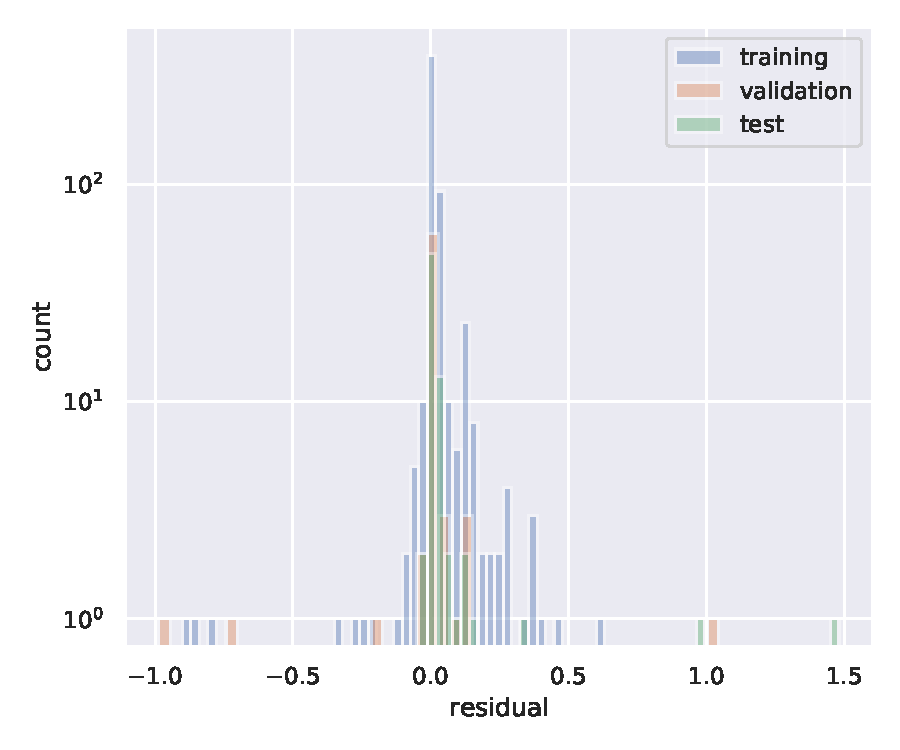
\includegraphics[width=\linewidth]{img/lumps_ann_residual_histogram_compare}
    \caption{Residuals.}
  \end{subfigure}
  \hfill
  \begin{subfigure}[b]{0.45\linewidth}
    \centering
    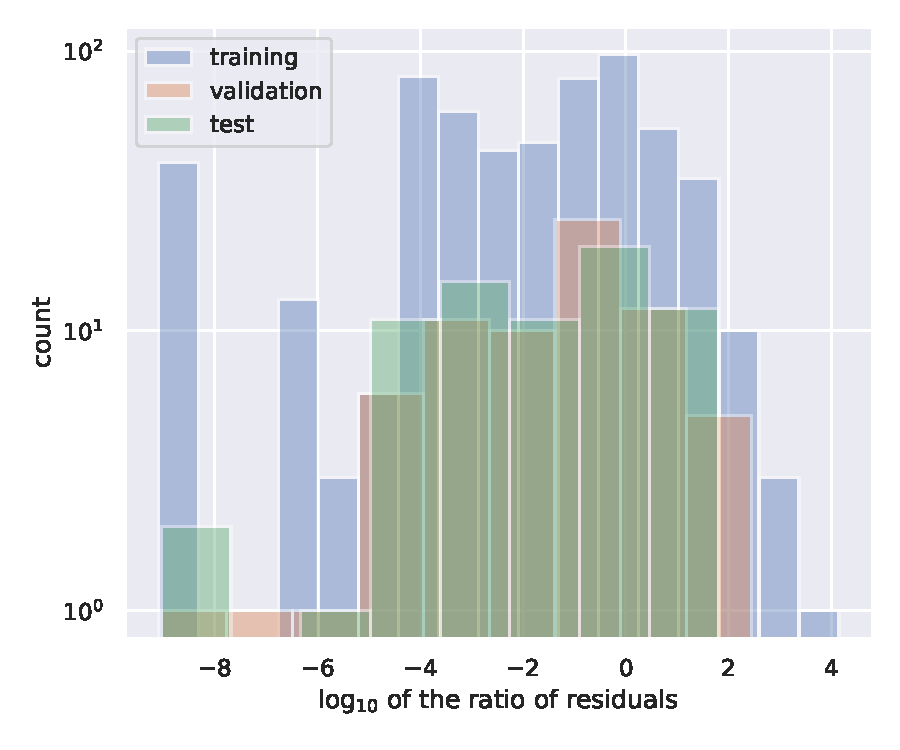
\includegraphics[width=\linewidth]{img/lumps_ann_ratio_histogram_compare}
    \caption{Ratio of the predicted and final residuals.}
  \end{subfigure}
  \caption{Univariate distributions of the residuals using the ANN model on the full dataset.}
  \label{fig:lumps:fftann}
\end{figure}


In~\Cref{tab:lumps:fftres} we show the results obtained on the test fold using the full dataset.
It seems that while the GBDT reach a better \mse result, SVR succeeds in improving the ratio of the residuals with respect to the finite approximation.
Overall the neural network was able to achieve the best results, shown in~\Cref{fig:lumps:fftann}.

As a comparison we also trained the same algorithms on different subsamples of the dataset.
In~\Cref{tab:lumps:fftres_type2} we show the results on the test set obtained by selecting only \texttt{type} $= 2$ samples.\footnotemark{}
\footnotetext{%
  The selection is made prior to subdividing the dataset into training and test sets, thus also the test fold is made of samples of the same \texttt{type}.
}
In~\Cref{tab:lumps:fftres_type4} we instead show the results on the test set obtained with \texttt{type} $= 4$ samples.\footnotemark{}
\footnotetext{%
  As in the previous case, the selection is made before splitting the dataset.
}
We therefore see that the most problematic samples are usually in the \texttt{type} $= 4$ subset, where the largest improvements on the ratio of the residuals are made.
However the \texttt{type} $= 2$ is remarkably well approximated by linear functions.
In both cases the ANN showed great improvements in the predictions with respect to the approximation using finite truncation levels.

\begin{table}[htbp]
  \centering
  %\resizebox{\textwidth}{!}{%
  \begin{tabular}{@{}ccccc@{}}
       \toprule
       & \mse & \mae & \rr & R \\
       \midrule
    LR   & \num{7.0e-6} & \num{2.0e-3} & 1.00 & -0.13 \\
    SVR  & \num{1.6e-5} & \num{2.9e-3} & 1.00 & -0.07 \\
    GBDT & \num{3.0e-4} & \num{8.9e-3} & 1.00 & 0.16  \\
    ANN  & \num{7.0e-8} & \num{2.0e-4} & 1.00 & -1.25 \\
       \bottomrule
  \end{tabular}%
  %}
  \caption{%
    Predictions of the \ml analysis trained on \texttt{type} $= 2$ samples.
    Results refer to the test fold.
  }
  \label{tab:lumps:fftres_type2}
\end{table}

\begin{table}[htbp]
  \centering
  %\resizebox{\textwidth}{!}{%
  \begin{tabular}{@{}ccccc@{}}
       \toprule
       & \mse & \mae & \rr & R \\
       \midrule
    LR   & 0.23 & 0.36 & 0.51  & -1.00 \\
    SVR  & 0.03 & 0.05 & 0.94  & -2.42 \\
    GBDT & 0.47 & 0.65 & -0.02 & -0.63  \\
    ANN  & 0.03 & 0.03 & 0.94  & -3.18 \\
       \bottomrule
  \end{tabular}%
  %}
  \caption{%
    Predictions of the \ml analysis trained on \texttt{type} $= 4$ samples.
    Results refer to the test fold.
  }
  \label{tab:lumps:fftres_type4}
\end{table}


\subsubsection{Signal Processing and LSTM Network}

As an additional analysis we also processed the truncation levels as subsequent approximations of the extrapolated labels.
We therefore used a \emph{Long Short-Term Memory} (LSTM) neural network to study the finite truncation levels as signals reaching the \texttt{exp} labels.\footnotemark{}
\footnotetext{%
  LSTM networks are for instance used in making financial or atmospheric predictions using a series of data.
}
In the first straightforward approach we used the unprocessed truncation levels and directly predicted the \texttt{exp} label using a single LSTM network.
We then compared the results with the same process after feature engineering: we first applied a Fourier transform to the levels and then compute the predictions by combining two LSTM networks separately processing the complex modulus and the argument angle of the Fourier transformed levels.
In both cases we drop the categorical \texttt{type} and the \texttt{weight} variables and use only the truncation levels.

The first model used is made of \num{4} bidirectional LSTM layers with \numlist{50;30;30;10} units each (we used the default activations to be able to use the \texttt{cuDNN} acceleration provided by the framework).
We used $10^{-2}$ $\ell_2$ regularisation in the first two layers and $10^{-3}$ in the last two hidden layers.
We also implemented dropout layers with $0.2$ dropout rate in the first two layers and $0.1$ in the last two.
The model was finally compiled with the \texttt{Adam} optimizer with an initial learning rate of $0.001$.
We then scheduled the learning rate to reduce as in~\eqref{eq:lumps:lrschedule}.
As in the previous cases an early stopping techniques was used to halt training after \num{2500} epochs without improving of the \mse, used as loss function.

The second model is formed by two sub-architectures mirroring the same layers, regularisation and dropout as the first model.
One of the sub-architectures is then fed the complex modulus of the Fourier transformed truncation levels while the other takes the angles as input.
The two sub-architectures are then concatenated before outputting a single predicted labels as in~\Cref{fig:lumps:lstm}.
The entire model is then trained as supervised task on the \texttt{exp} labels.

\begin{figure}[htbp]
  \centering
  \begin{subfigure}[b]{0.45\linewidth}
    \centering
    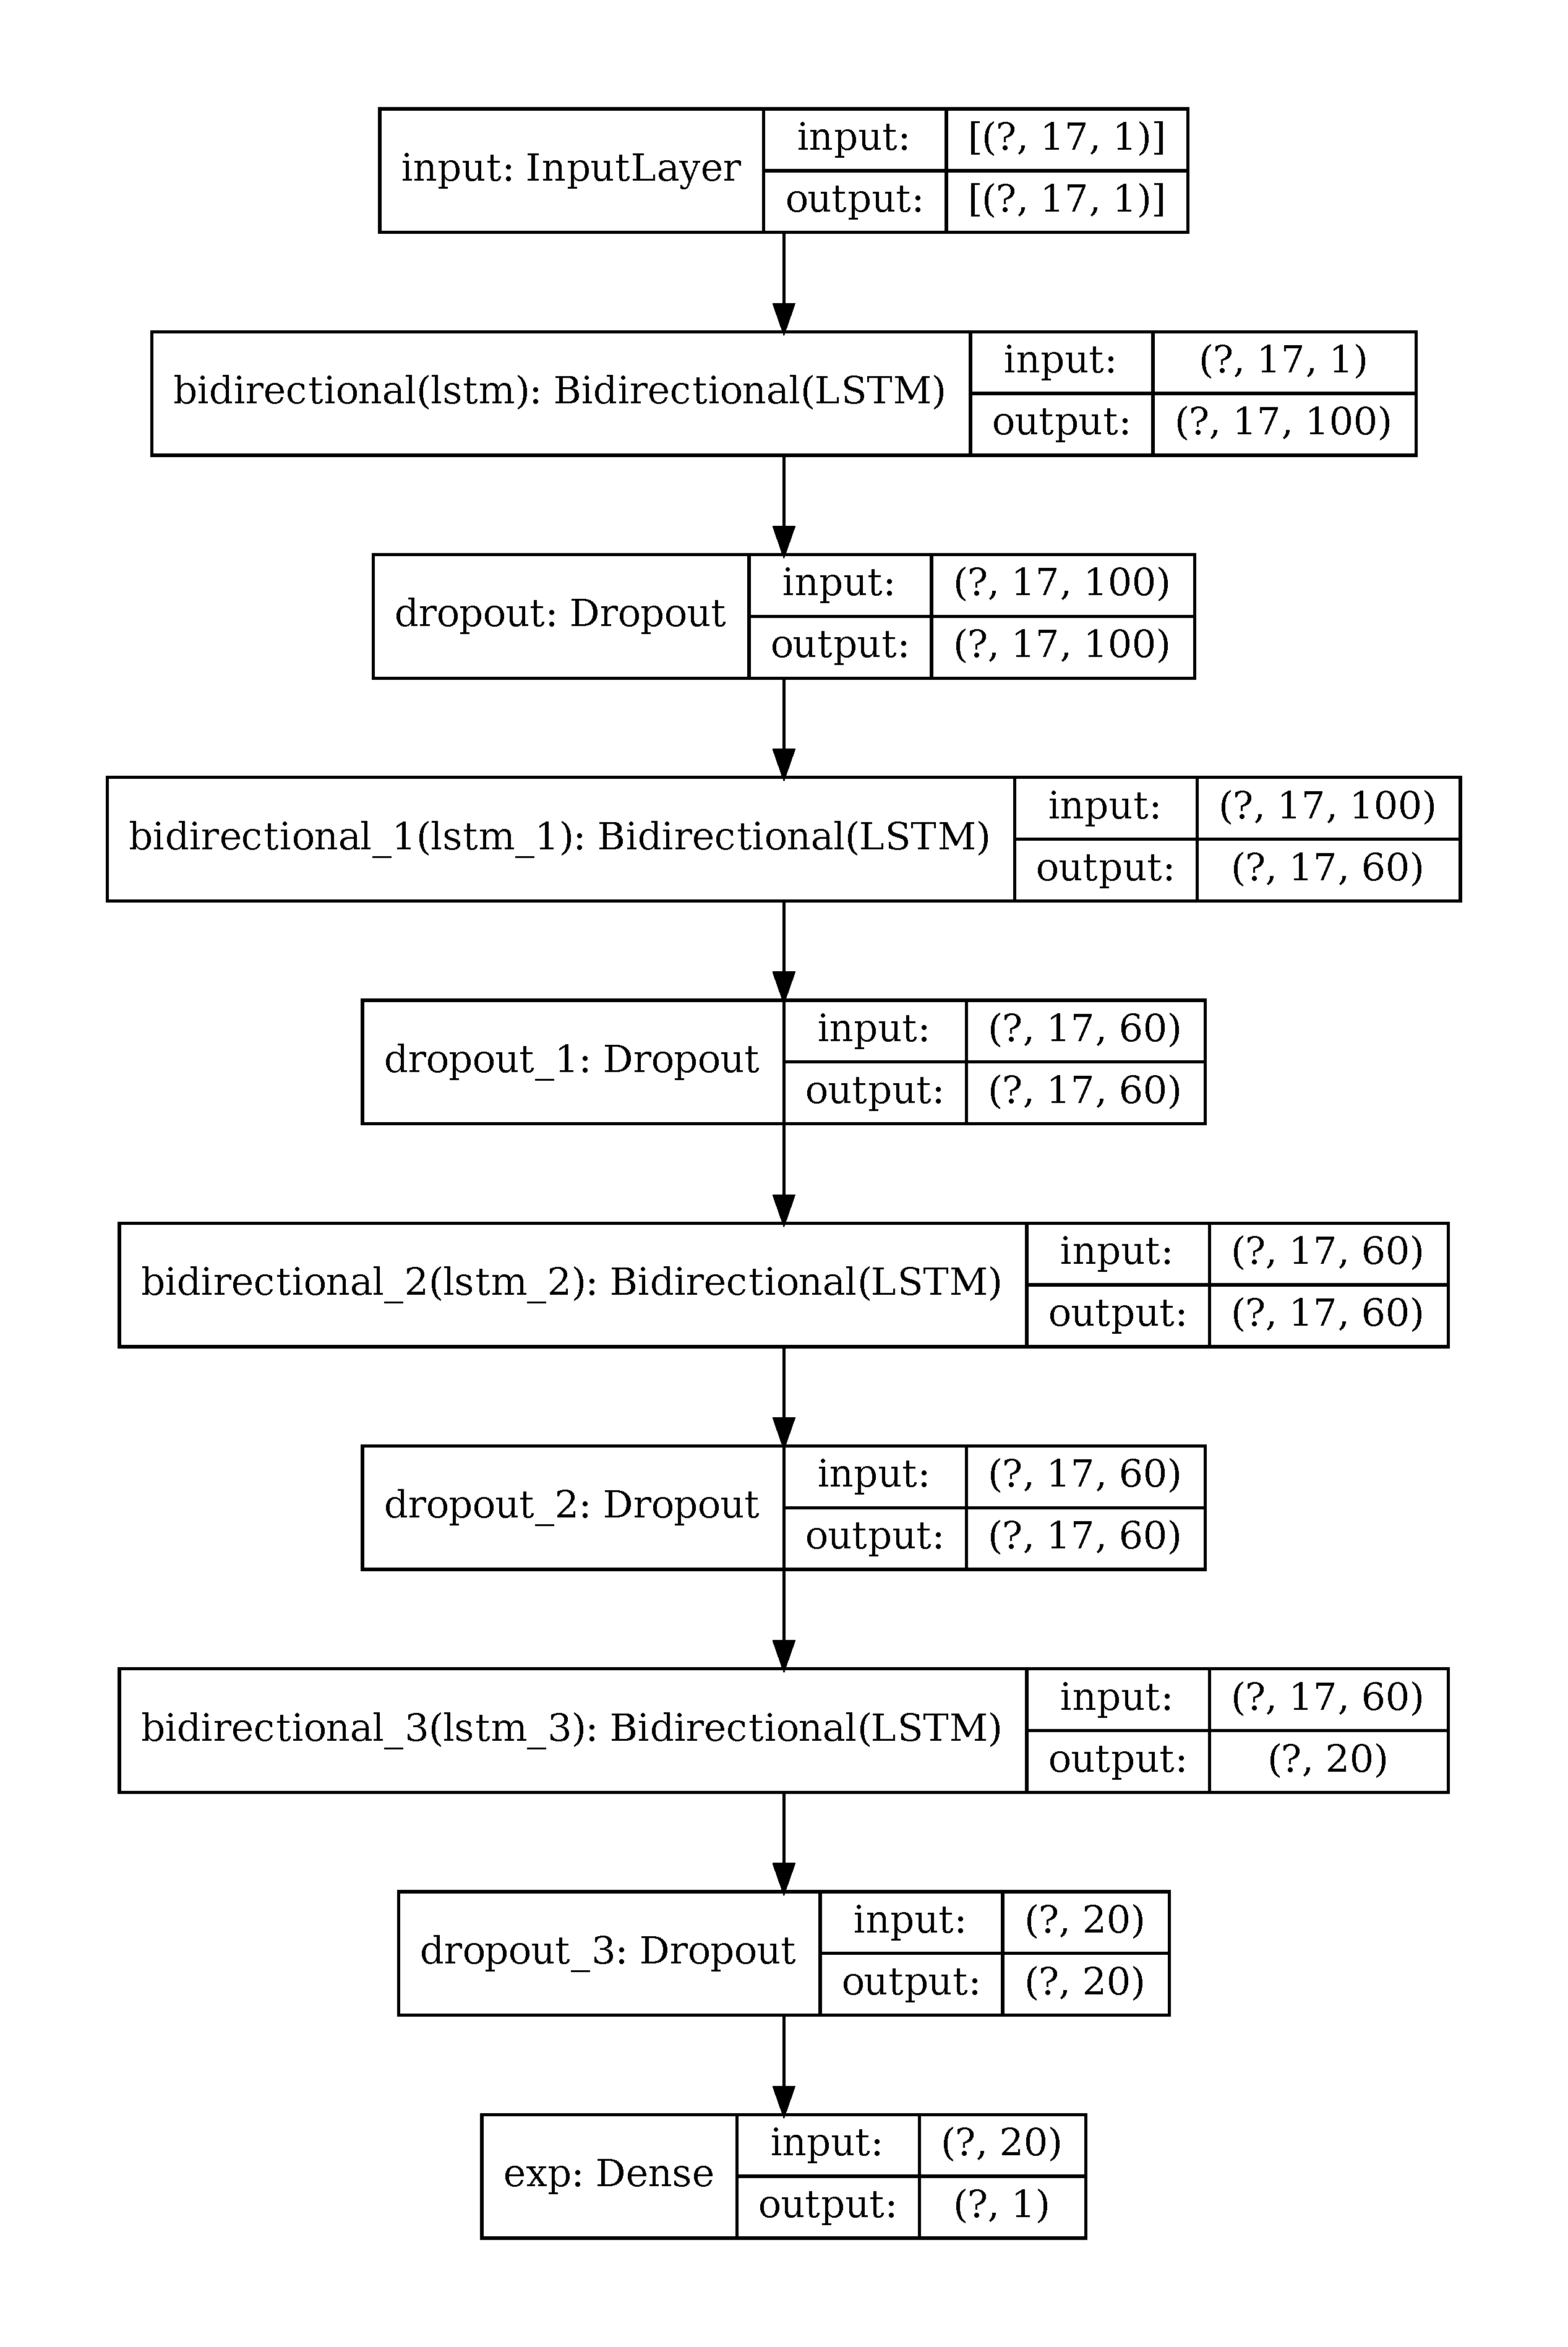
\includegraphics[height=0.95\linewidth]{img/lumps_ann_arch_lstm}
    \caption{Straightforward model.}
  \end{subfigure}
  \hfill
  \begin{subfigure}[b]{0.45\linewidth}
    \centering
    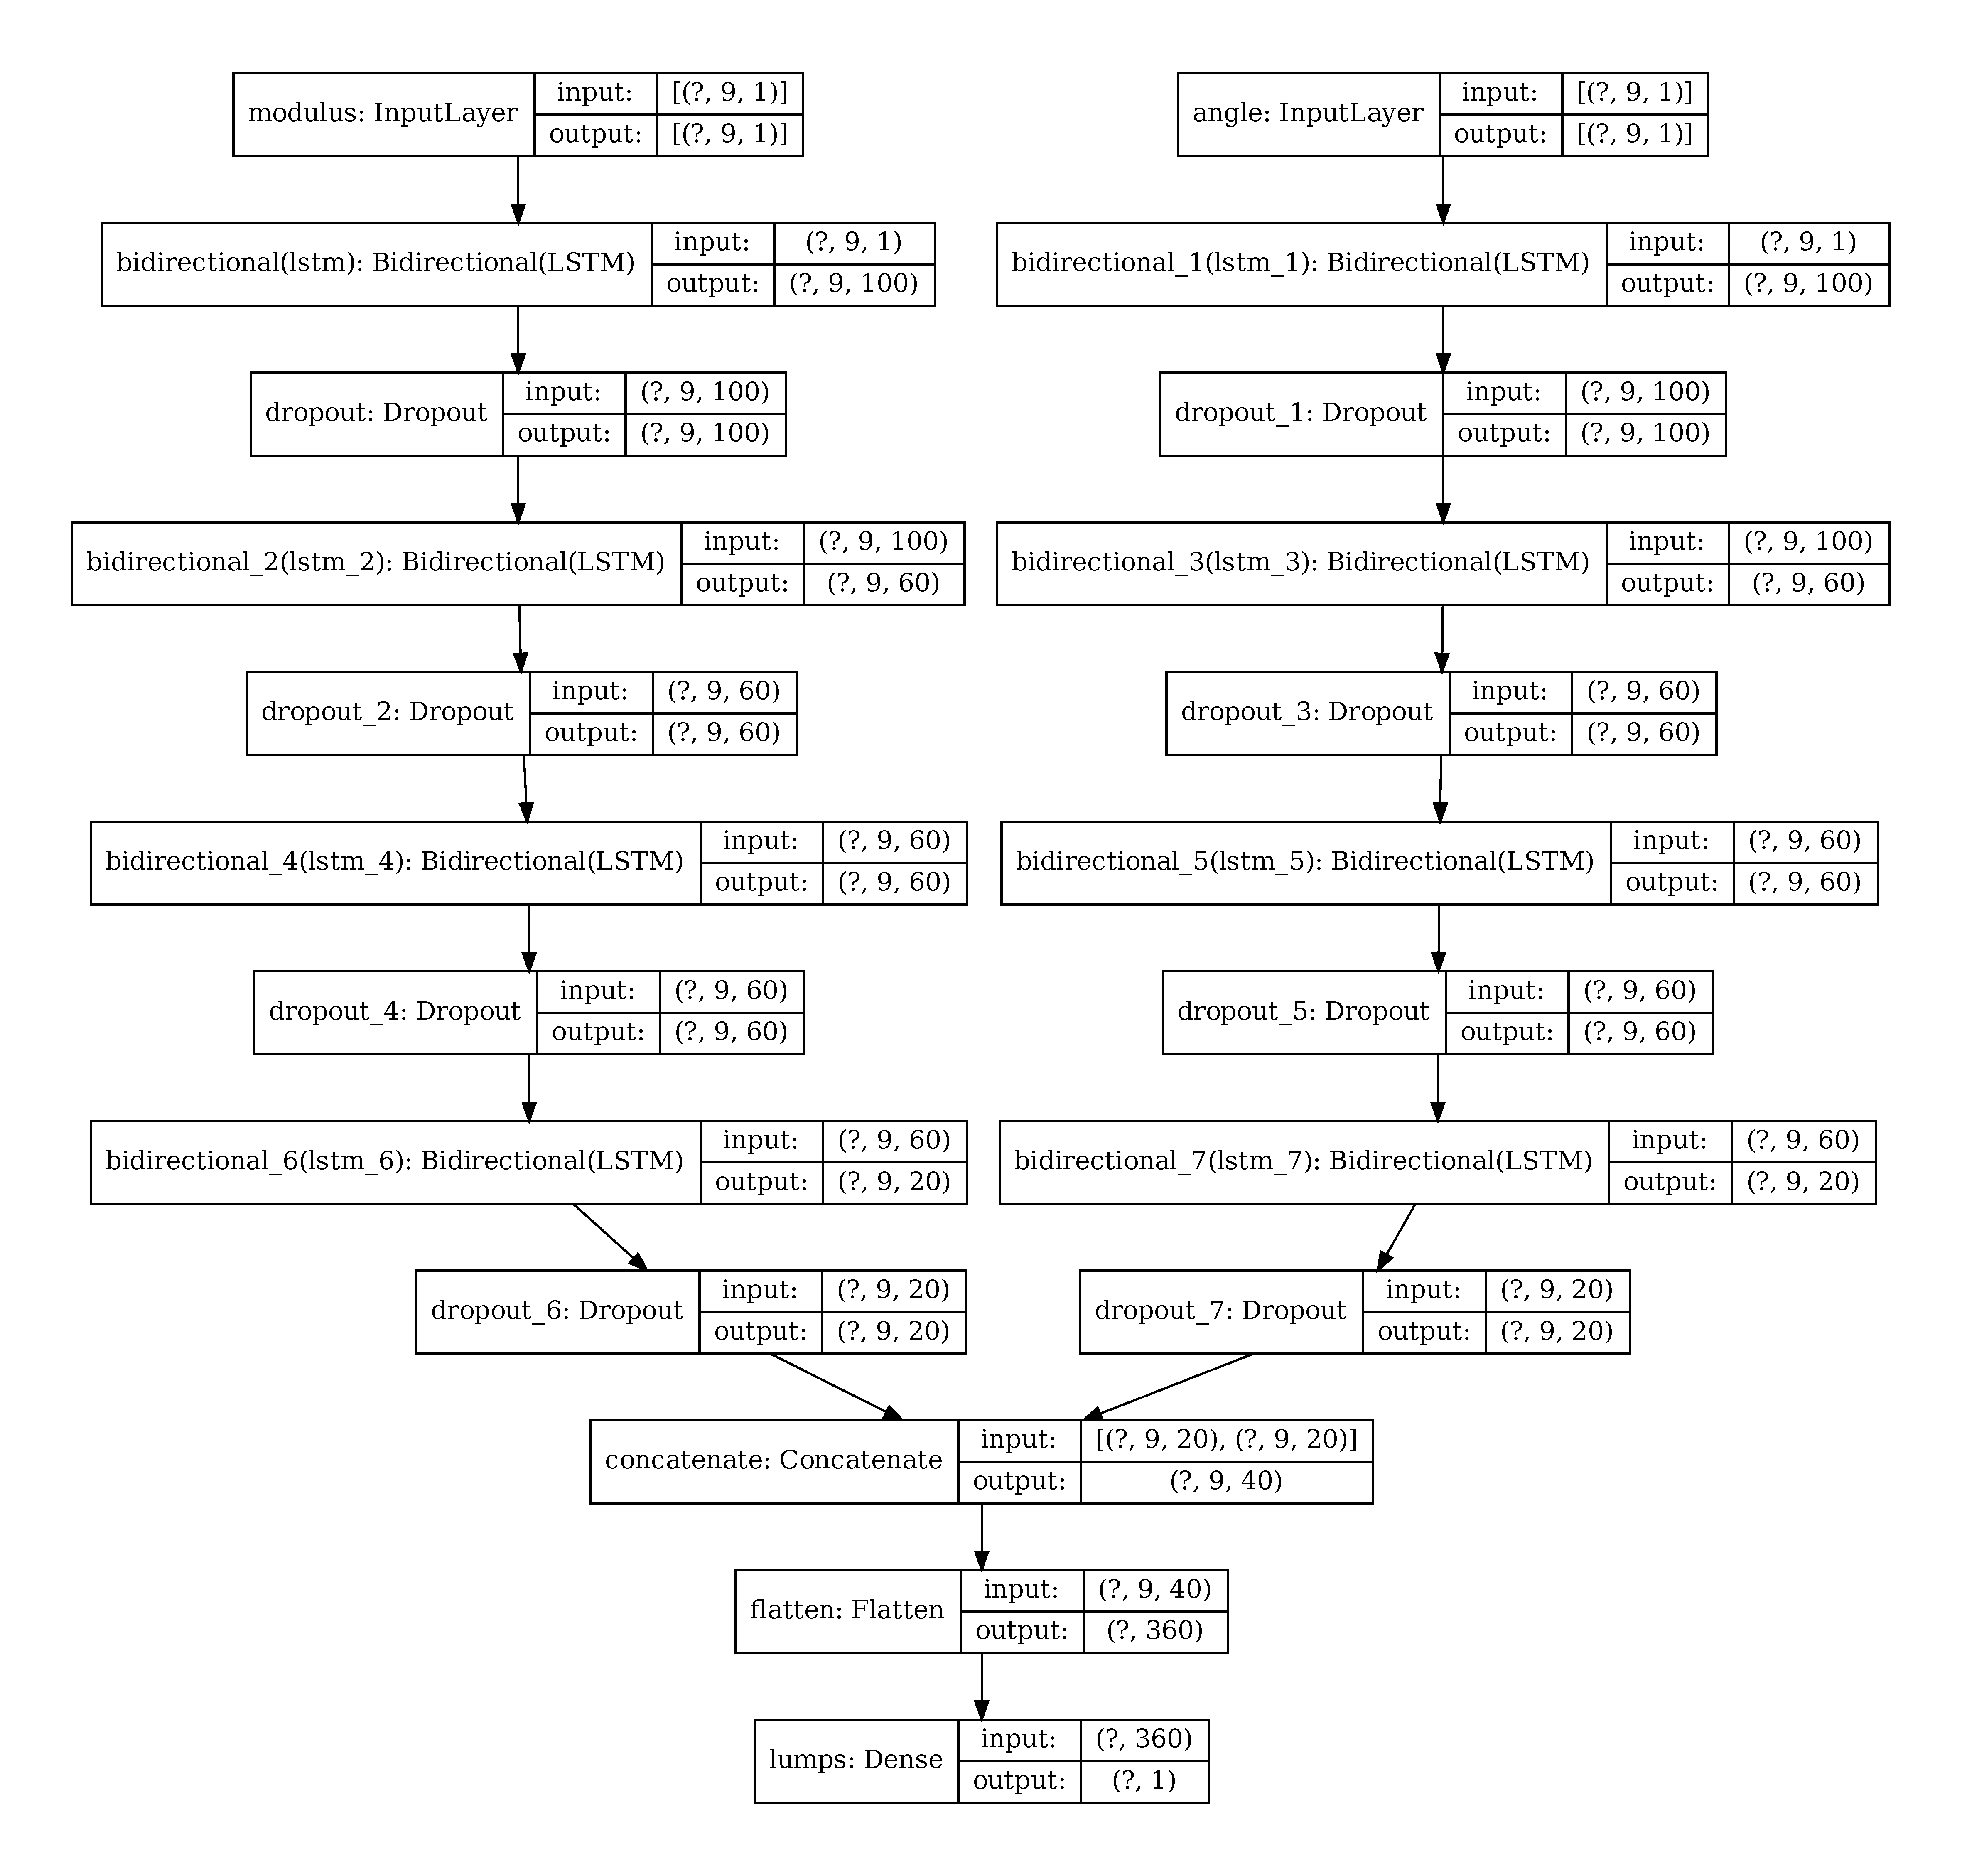
\includegraphics[height=0.95\linewidth]{img/lumps_ann_arch_lstm_fft}
    \caption{Fourier transformed model.}
  \end{subfigure}
  \caption{LSTM models used in the analysis.}
  \label{fig:lumps:lstm}
\end{figure}

In~\Cref{tab:lumps:lstm} we show the metrics computed using the LSTM networks as described.
It seems that using just the truncation levels can actually provide insightful information without using the weight or the oscillation type of the observables.
In fact using the Fourier transformed truncation levels provides a non negligible average improvement on the ratio of the residual errors.

\begin{table}[htbp]
  \centering
  %\resizebox{\textwidth}{!}{%
  \begin{tabular}{@{}ccccc@{}}
       \toprule
       & \mse & \mae & \rr & R \\
       \midrule
    LSTM        & 0.88 & 0.79 & -1.22 & -0.11 \\
    LSTM + FFT  & 0.25 & 0.24 & 0.36  & -1.36 \\
       \bottomrule
  \end{tabular}%
  %}
  \caption{%
    Predictions of the test fold using the LSTM networks.
  }
  \label{tab:lumps:lstm}
\end{table}


\subsubsection{Double Lumps Inference}

Using the previously trained algorithms we can also try to infer the results of the double lumps.
For predictions we use only entries such that \texttt{weight} $\le 1.25$ since they represent the most reliable ground truth values available.
In~\Cref{tab:lumps:dlumpsres} we show the predictions made on the subset of double lumps observables using the previously trained algorithms.
We also provide the result obtained by using the last finite truncation level as a comparison.
Notice that in order to get to these results we multiplied the output of the \ml models by a factor \num{2}.

\begin{table}[htbp]
\centering
\resizebox{\textwidth}{!}{%
  \begin{tabular}{@{}cccccccccc@{}}
    \toprule
    \texttt{weight} & \texttt{type} & \texttt{exp} & \texttt{level\_18} & \textbf{LR} & \textbf{r-SVR} & \textbf{GBDT} & \textbf{ANN (FC)} & \textbf{LSTM} & \textbf{LSTM + FFT} \\
    \midrule
    0.0             & 2             & 2.000132     & 2.010872           & 0.739581    & -5.195649    & 1.029453      & 1.977009          & 1.753636      & 1.983604            \\
    0.0             & 2             & -0.000045    & 0.000039           & 0.725948    & -17.250588   & 1.252845      & 1.834650          & 0.317282      & -0.108339           \\
    1.0             & 4             & -2.000161    & -2.048203          & -0.526719   & 0.924571     & -0.737725     & -0.029497         & -0.357706     & -2.057807           \\
    0.0             & 4             & 1.998589     & 2.008174           & 0.966371    & 1.449645     & 1.557821      & 1.961694          & 1.752006      & 1.951245            \\
    0.027778        & 4             & 0.955293     & 0.875055           & 1.689489    & 1.045768     & 1.506691      & 1.976213          & -0.422734     & 1.990272            \\
    0.111111        & 4             & -1.083093    & -1.174038          & 1.025812    & 1.427613     & 1.596725      & 1.954148          & 1.631063      & -0.084639           \\
    0.25            & 4             & -1.994476    & -1.952275          & 0.415141    & 1.045758     & 0.815447      & 1.998802          & -0.069527     & 1.677992            \\
    0.444444        & 4             & -0.827465    & -0.573408          & 0.083566    & 1.045758     & 0.818691      & 1.976839          & 0.556283      & 1.897519            \\
    0.694444        & 4             & 1.213654     & 1.409107           & 1.038451    & 1.045758     & 2.078447      & 2.027592          & 0.224882      & 1.948670            \\
    0.0             & 4             & 2.015004     & 1.585226           & 1.769235    & 1.045763     & 1.657983      & 2.097705          & 0.357322      & 1.990428           \\
    \bottomrule
\end{tabular}%
}
\caption{%
  Predictions of the double lumps using trained algorithms.
  Every prediction has been scaled (mulitplied) by a factor 2 to reach the values shown in the table.
  ANN refers to the fully connected (FC) model, while the LSTM network are divided into real and complex inputs.
}
\label{tab:lumps:dlumpsres}
\end{table}

As we can see both from the results and the metrics~\Cref{tab:lumps:dlumpsmet} using the lumps dataset is not enough to reproduce also the double lumps.
In fact even by scaling the results we did not get a satisfactory result.
The LSTM network using the Fourier transformed layers proved to work slightly better, but the result is still worse than using the finite truncation levels ($R > 0$).
The difference between lumps and double lumps is therefore not just a scale factor.
In fact the distributions of the variables are quite different in the two datasets.

\begin{table}[htbp]
  \centering
  %\resizebox{\textwidth}{!}{%
  \begin{tabular}{@{}ccccc@{}}
    \toprule
                & \mse & \mae & \rr   & R \\
    \midrule
    LR          & 1.7  & 1.1  & 0.28  & 1.40  \\
    r-SVR       & 37   & 3.7  & -15.0 & 1.6   \\
    GBDT        & 2.3  & 1.3  & 0.02  & 1.48  \\
    ANN (FC)    & 4.2  & 1.6  & -0.8  & 1.2   \\
    LSTM        & 2.2  & 1.3  & 0.09  & 1.4   \\
    LSTM + FFT  & 2.4  & 0.9  & 0.01  & 0.85  \\
       \bottomrule
  \end{tabular}%
  %}
  \caption{%
    Metrics computed on the double lumps.
    ANN refers to the fully connected (FC) model, while LSTM models are separately reported for both purely real and complex input.
  }
  \label{tab:lumps:dlumpsmet}
\end{table}


\subsubsection{Other Analyses and Complementary Data}
\label{sec:lumps:other}

As complementary analyses and comparison there are other notebooks available on \href{https://github.com/thesfinox/ml-sft-trunc/tree/model-dep}{GitHub}.
As a matter of fact we studied also the predictive ability of the models under different circumstances:
\begin{itemize}

  \item selecting only conformal invariant observables (i.e.\ \texttt{weight} $= 0$) showing that in general predictions on these observables are more accurate as the distribution of the data is less affected by outliers,
  
  \item selecting separately \texttt{type} $= 2$ and \texttt{type} $= 4$ observables (in general \texttt{type} $= 2$ implies \texttt{weight} $= 0$ and it is easier to study),

  \item taking only \texttt{weight} $\le 1.25$ showing that higher weights are in general much more difficult to handle,
    
  \item selecting only ``good'' behaving observables (i.e.\ taking only observables whose absolute difference between \texttt{level\_18} approximations and \texttt{exp} are $\le 0.1$), showing that \ml can still make some improvements,

\end{itemize}
Other LSTM architecture have also been explored by taking only ``good'' behaving observables and by including an initial \emph{embedding} layer made of fully connected layer as preprocessing techniques before feeding the recurrent network.



% vim ft=tex
